\documentclass[dvipdfmx,openany,uplatex]{jsbook}
\usepackage[deluxe,multi,jis2004]{otf}              % 多書体フォント対応(JIS2004拡張漢字対応)
\usepackage[dvipdfmx]{graphicx}                     % 画像表示
\usepackage{amsmath, amssymb, amsfonts, mathtools}  % 数式表示
\usepackage{amsthm}                                 % 定理表示
\usepackage[dvipdfmx]{hyperref}                     % 参考文献リンク
\usepackage{subcaption}                             % 小さいキャプション
\usepackage{url}                                    % url表示
\usepackage{enumerate}                              % 箇条書き
\usepackage{ascmac}                                 % 枠囲み
\usepackage{tcolorbox}                              % 枠囲み(プロンプト部分)
\usepackage{listings,jvlisting}                     % ソースコード表示
\usepackage{algpseudocode}                          % 疑似コード表示
\usepackage{algorithm}                              % アルゴリズム表示
\usepackage{booktabs}                               % 表の罫線
\usepackage{multirow}                               % 表のセル結合
\usepackage{tabularx}                               % 可変幅の表
\usepackage{siunitx}                                % 数値・単位の表示
\usepackage{diagbox}                                % 表のセル斜線分割
\usepackage{tikz}                                   % 図描画

\usetikzlibrary{arrows.meta,positioning}
\tcbuselibrary{breakable}
% \usepackage[dvipdfmx]{xcolor}                   % 参考文献リンク

\newcommand{\bhline}[1]{\noalign{\hrule height #1}}
\addtolength{\fullwidth}{-26truemm}  % 全体の幅(ヘッダ部の幅)を既定値から26mm小さくする
\setlength{\textwidth}{\fullwidth}   % 本文の幅(textwidth)を全体の幅(=ヘッダ部の幅)にそろえる
\setlength{\evensidemargin}{1truemm} % 偶数ページの左余白を1mm(+1インチ)にする
\setlength{\oddsidemargin}{19truemm} % 奇数ページの左余白を19mm(+1インチ)にする
\numberwithin{equation}{section}     % 式番号を(1.〇)で表示する
\setcounter{tocdepth}{2}             % subsubsectionまで目次に表示する

%%% ソースコード表示の設定 %%%
\lstset{
  basicstyle={\ttfamily},
  identifierstyle={\small},
  commentstyle={\smallitshape},
  keywordstyle={\small\bfseries},
  ndkeywordstyle={\small},
  stringstyle={\small\ttfamily},
  frame={tb},
  breaklines=true,
  columns=[l]{fullflexible},
  numbers=left,
  xrightmargin=0zw,
  xleftmargin=3zw,
  numberstyle={\scriptsize},
  stepnumber=1,
  numbersep=1zw,
  lineskip=-0.5ex
}
\renewcommand{\lstlistingname}{コード}

%%%% 表紙用設定 %%%%
\hoffset0mm
\voffset0mm
\makeatletter
\let\@@shipout\shipout
\def\shipout\vbox{\@@shipout\vbox\bgroup\afterassignment\insertBackGround\let\reserved@a=}
\def\insertBackGround#1{#1%
        \iftombow
                \copy\BackGround\kern0pt
        \else
                \kern-1truein\moveleft1truein\copy\BackGround\kern1truein
        \fi}
\newbox\BackGroundUnit
\newbox\BackGround
\def\@haikei#1{
\setbox\BackGroundUnit\hbox{\includegraphics*[width=\paperwidth]{#1}}
\@tempdima\paperheight
\advance\@tempdima\ht\BackGroundUnit\advance\@tempdima\dp\BackGroundUnit
\setbox\BackGround\vbox to \@tempdima{
        \@tempdima=\paperwidth\advance\@tempdima\wd\BackGroundUnit
        \leaders\hbox to\@tempdima{\leaders\copy\BackGroundUnit\hfil}\vfil
}
\wd\BackGround=0pt\ht\BackGround=0pt\dp\BackGround=0pt
}
\newcommand{\incluedefullgraphics}[1]{\pagestyle{empty}\@haikei{#1}\null}
\makeatother
%%%%%%%%%%%%%%%%%%%%

\begin{document}
\begin{titlepage}
  \thispagestyle{empty}
  \incluedefullgraphics{cover.png}
\end{titlepage}

\chapter*{はじめに}
本誌を手に取ってくださり、ありがとうございます。
京都大学人工知能研究会 KaiRA 会長の岡本和優です。

\vskip\baselineskip

人工知能という言葉は、いまや特別な響きをもたなくなりました。
つい数年前——GPT-2がその安全性の懸念から一般公開すらされていなかった頃は、AIは研究室や巨大企業だけが扱う「特別な道具」でした。
それが今では、インターネットさえつながっていれば、誰もがAIを使ったサービスを利用でき、日常の中に自然に溶け込むようになっています。

\vskip\baselineskip

AI を「使う」ことについては確かに民主化が進みましたが、AI を「作る」「研究する」側の世界は、まだ十分に開かれているとは言えません。
巨大企業だけが膨大な計算資源を用いてモデルを訓練し、研究の主導権はますます閉じた領域に集中しています。
かつてオープンであると信じられたAI研究の世界は、気づけばマネーゲームの世界へと収束しつつあります。

だからこそ、私たちのような小さなコミュニティが、自分たちの手で考え、試し、つくってみることに意味があります。
シンギュラリティが来るかどうかといった大きな議論よりも、まずは自分たちの身近な問いから技術を生み出し、
ほんの少しでも未来をよくする試みを続けていくこと——それこそが、AI時代の創造性だと私は思っています。

大規模モデルが世界を塗り替えようとしている今でも、「自分たちで未来を形にしよう」とする学生たちの活動は決して色あせません。
むしろ、この時代だからこそ、その小さな挑戦には大きな価値があるのではないでしょうか。

\vskip\baselineskip

本誌には、学生が主体となって取り組んだ研究や開発の記録が収められています。
そこに書かれているのは、華やかな成功ばかりではありません。しかし、そこで生まれた「試行錯誤の跡」こそが、この会誌の魅力です。

どんな問いを持ち、どう試して、どこでつまずき、何を得たのか。
そのひとつひとつが、これからの技術や研究につながる小さな種だと思っています。

読者のみなさんには、ぜひこの 「挑戦のプロセス」 を楽しんでいただければ幸いです。
巨大資本や巨大モデルが主導する時代だからこそ、
学生が自分の興味や疑問から始めた小さな試みには、ほかにはない輝きがあると信じています。

\vskip\baselineskip
\rightline{京都大学人工知能研究会KaiRA\ 会長}
\rightline{岡本和優}
\rightline{2025年11月吉日}

\tableofcontents

\chapter{ニューラルネットワーク入門}\label{chap:nn-intro}
\section{はじめに}
近年の人工知能(AI)の目覚ましい発展は、まさに「ニューラルネットワーク」という技術によって牽引されてきました。スマートフォンが顔を認識したり、音声アシスタントが言葉の意味を理解したり、あるいはAIが美しい絵画や自然な文章を生成したり――私たちが日常で「すごい」と感じるAIの多くが、このニューラルネットワークを基盤として動いています。

とはいえ、「ニューラルネットワーク」と聞くと、難解な数式や複雑な理論を思い浮かべてしまう人も少なくないでしょう。

でも、安心してください。本稿の目的は、数学的な細部に立ち入ることではありません。私たちが共有したいのは、この技術の「どこが面白いのか」、そして「なぜここまで強力なのか」という「直感」です。

本稿は、\textbf{「AI という言葉は知っているが、体系的に学んだことはない」}という方に向けた、やさしい入門ガイドです。専門的な知識がなくても読み進められるよう、基本的な概念から丁寧に解説していきます。

\section{生物の神経細胞から着想を得たモデル}
ニューラルネットワークの最初のアイデアは、非常にシンプルで、私たちの身近にあるものから着想を得ています。それは、生物の脳に存在する\textbf{ニューロン(神経細胞)}です。

私たちの脳内では、ニューロンが複雑なネットワークを形成しています。個々のニューロンは、他のたくさんのニューロンから電気的な信号を受け取ります。そして、受け取った信号の合計が、ある一定の「しきい値(閾値)」を超えると、そのニューロンは「発火(興奮)」し、次のニューロンへと今度は自らが信号を送るのです。

この仕組みを、ごくごくシンプルに数学的なモデルとして置き換えてみましょう。

\begin{enumerate}
    \item 複数の入力(信号)を受け取る。
    \item それらを合計する。
    \item 合計が「しきい値」を超えたら「1」(発火)を、超えなければ「0」(発火しない)を出力する。
\end{enumerate}

たったこれだけです。これが、人工ニューラルネットワークの原点であり、出発点です。

ここで重要な直感が生まれます。私たちの「知能」や「記憶」は、決して一つの万能なニューロンが担っているわけではありません。むしろ、比較的単純な働きをする「多数の素朴な処理ユニット」が、お互いに結びつき、チームとして連携することで、全体として非常に高度な知性が生まれるのではないか、という考えです。

この「チームワーク」こそが知性の本質である、という考えは、生物学的な事実とも一致します。例えば、あるサッカーチームが1年間練習して強力なチームワークを築いたとします。もし急にメンバーの半分がルールも知らない素人と入れ替わったら、そのチームはガタガタになってしまいます。脳のニューロンが頻繁に入れ替わらないのは、この「チームワーク」、すなわちニューロン同士の安定した接続パターンこそが「記憶」や「知能」そのものだからです。

ニューラルネットワークも同じです。個々の「処理ユニット(人工ニューロン)」は単純でも、その「接続の仕方」や「連携の強さ(チームワーク)」を学習させることで、大きな知能が生まれるのです。

\section{パーセプトロン:最初のニューラルネットワーク}
この「脳の神経細胞(ニューロン)」の仕組みを、世界で初めて工学的にモデル化したものが、1950年代に考案された「パーセプトロン」です。これは、まさにAIの「ご先祖様」と呼べる存在です。

パーセプトロンの仕組みは、先ほどのニューロンのモデルとほぼ同じです。複数の入力に対し、それぞれ「重み」をかけて合計し、その値が「しきい値(あるいはバイアス)」を超えたら1、そうでなければ0を出力します。

\begin{figure}[H]
  \centering
  \begin{tikzpicture}[
    >=Stealth,
    node distance=2.2cm,
    every node/.style={font=\normalsize}
  ]
    % ノード
    \node[circle, draw, minimum size=10mm] (sum) {$\sum$};
    \node[draw, rounded corners, right=3cm of sum, minimum height=10mm, minimum width=16mm] (act) {$\varphi(\cdot)$};
    \node[right=2.5cm of act] (y) {$y$};

    % 入力(x1, x2, ..., xn)
    \node[left=4.2cm of sum, yshift=12mm] (x1) {$x_{1}$};
    \node[left=4.2cm of sum, yshift=4mm]  (x2) {$x_{2}$};
    \node[left=4.2cm of sum, yshift=-12mm] (xn) {$x_{n}$};

    % 省略記号
    \node[left=4.2cm of sum] (dots) {$\vdots$};

    % バイアス(1 → Σ, 重み b)
    \node[left=4.2cm of sum, yshift=-28mm] (one) {$1$};

    % 矢印(入力→Σ)
    \draw[->] (x1) -- node[above, pos=0.55] {$w_{1}$} (sum);
    \draw[->] (x2) -- node[above, pos=0.55] {$w_{2}$} (sum);
    \draw[->] (xn) -- node[above, pos=0.55] {$w_{n}$} (sum);
    \draw[->] (one) -- node[above, pos=0.55] {$b$} (sum);

    % Σ → 活性化 → 出力
    \draw[->] (sum) -- node[above] {$z=\sum_{i=1}^{n} w_i x_i + b$} (act);
    \draw[->] (act) -- (y);

  \end{tikzpicture}
  \caption{単一パーセプトロンの模式図(重み $w_i$,バイアス $b$,活性化 $\varphi$)}
  \label{fig:perceptron}
\end{figure}

ここで新しい言葉が2つ出てきました。「重み」と「しきい値(バイアス)」です。これらを簡単な例で考えてみましょう。

あなたが「今日は傘を持っていくべきか?」を判断する、シンプルなパーセプトロン(“傘判断”AI)になったと想像してください。

\begin{itemize}
    \item \textbf{入力}:
     
    入力1 $x_1$:「雨が降っているか?」(Yes=1, No=0)

    入力2 $x_2$:「天気予報が雨か?」(Yes=1, No=0)
    \item \textbf{重み}:
    
    「どの入力を、どれだけ重視するか」をコントロールする値です。

    重み1 $w_1$:「今、実際に降っている」(入力1)は非常に重要なので、重み5に設定。

    重み2 $w_2$:「予報」(入力2)は、まぁ重要だが外れることもあるので、重み2に設定。
    \item \textbf{しきい値(バイアス)}:

    「どれくらいで"発火"(傘を持つ)と決めるか」のボーダーラインです。

    あなたがとても慎重な人なら、しきい値を1に設定するかもしれません(予報が雨なだけで傘を持つ)。

    あなたが楽観的な人なら、しきい値を4に設定するかもしれません(予報だけでは持たず、実際に降ってきたら持つ)。
\end{itemize}

この「重み」や「しきい値」をデータ(過去の経験)から自動で調整(学習)できるようにしたのが、パーセプトロンの画期的な点でした。

しかし、この初期のパーセプトロンには大きな限界がありました。それは、「線形的にしか境界を引けない」という問題です。

先ほどの例のように、入力の“足し算”で判断できるシンプルな問題(これは「線形分離可能」と呼ばれます)は解けます。しかし、世の中の問題はもっと複雑です。

例えば、「入力1と入力2の“どちらか一方だけ”がYesの時に1(発火)になる」という、有名な「XOR問題」はこのパーセプトロンでは解けませんでした 。一本の直線では、この複雑な条件分けをどうやっても表現できなかったのです。

この“限界”の指摘は、当時のニューラルネット研究に大きな影響を与えました。もちろん、1960〜70年代に訪れた「AIの冬の時代」は、パーセプトロンの限界だけが原因ではありません。むしろ、ルールベースの記号処理AIが直面していた根本的な性能不足や計算資源の制約が、研究全体を停滞させた側面の方が大きかったと言われます。とはいえ、パーセプトロンではXORすら解けないという事実は、「より柔軟で表現力の高いモデルが必要だ」という強い問題意識を生み、のちの多層化──すなわち深層学習(ディープラーニング)へとつながる重要な伏線となりました。

\begin{figure}[H]
  \centering
  \begin{tikzpicture}[
    scale=3,
    every node/.style={font=\small}
  ]
    % 枠と座標軸
    \draw[->] (-0.1,0) -- (1.2,0) node[right] {$x_1$};
    \draw[->] (0,-0.1) -- (0,1.2) node[left] {$x_2$};
    \draw (0,0) rectangle (1,1);

    % 目盛り
    \foreach \x in {0,1}{
      \draw (\x,0) -- (\x,-0.03) node[right] {\x};
      \draw (0,\x) -- (-0.03,\x) node[left] {\x};
    }

    % XOR のデータ点
    % y=0:白抜き
    \draw[thick] (0,0) circle [radius=0.045];
    \draw[thick] (1,1) circle [radius=0.045];
    % ラベル(点と重ならないようアンカーで配置)
    \node[anchor=north east] at (0,0) {$\;y=0$};
    \node[anchor=south west] at (1,1) {$\;y=0$};

    % y=1:塗りつぶし
    \fill (1,0) circle [radius=0.045];
    \fill (0,1) circle [radius=0.045];
    % ラベル
    \node[anchor=north west] at (1,0) {$\;y=1$};
    \node[anchor=south east] at (0,1) {$\;y=1$};

    % 任意の直線(例示)
    \draw[dashed] (-0.1,0.7) -- (1.2,0.2);

  \end{tikzpicture}
  \caption{XOR の例:対角に異なるクラスが配置され、どの直線でも完全に分離できない(線形分離不可能)}
  \label{fig:xor_not_linearly_separable}
\end{figure}

\section{多層パーセプトロン(MLP)と深層学習の基本}
パーセプトロンの「XOR問題」という壁。この限界を乗り越えるために生まれたのが、\textbf{多層パーセプトロン(MLP: Multi-Layer Perceptron)}です。

アイデアは、構造を「多層化」することでした。

パーセプトロンが「入力層」と「出力層」だけだったのに対し、MLPはその間に\textbf{「隠れ層(Hidden Layer)」}と呼ばれる新しい層を挿入しました。

\begin{figure}[H]
  \centering
  \begin{tikzpicture}[
    >=Stealth,
    neuron/.style={circle, draw, minimum size=9mm},
    every node/.style={font=\small},
    conn/.style={->, shorten >=1pt, shorten <=1pt}
  ]

    %=== X(横位置) ===%
    \def\xin{0}
    \def\xhid{4}
    \def\xout{8}

    %=== 入力層(縦配置) ===%
    \node[neuron] (x1) at (\xin,  2.4) {$x_1$};
    \node[neuron] (x2) at (\xin,  0.8) {$x_2$};
    \node[neuron] (x3) at (\xin, -0.8) {$x_3$};
    \node            at (\xin, -2.0) {$\vdots$};
    \node[neuron] (xn) at (\xin, -3.2) {$x_n$};

    % 層タイトル(被らないよう十分上に)
    \node[font=\bfseries] at (\xin, 3.25) {入力層};

    %=== 隠れ層(1層) ===%
    \node[neuron] (h1) at (\xhid,  2.0) {$h_1$};
    \node[neuron] (h2) at (\xhid,  0.7) {$h_2$};
    \node[neuron] (h3) at (\xhid, -0.6) {$h_3$};
    \node            at (\xhid, -1.8) {$\vdots$};
    \node[neuron] (hm) at (\xhid, -3.0) {$h_m$};

    \node[font=\bfseries] at (\xhid, 3.25) {隠れ層(活性化 $\varphi$)};

    %=== 出力層 ===%
    \node[neuron] (y)  at (\xout, 0.7) {$y$};
    \node[font=\bfseries] at (\xout, 3.25) {出力層};

    %=== 入力→隠れ(全結合) ===%
    \foreach \xinode in {x1,x2,x3,xn}{
      \foreach \hnode in {h1,h2,h3,hm}{
        \draw[conn] (\xinode) -- (\hnode);
      }
    }

    %=== 隠れ→出力(全結合) ===%
    \foreach \hnode in {h1,h2,h3,hm}{
      \draw[conn] (\hnode) -- (y);
    }

    %=== ラベル(図のさらに上に逃がす) ===%
    \node at ({(\xin+\xhid)/2}, 3.85)
      {全結合層( $W^{(1)}$, $b^{(1)}$)};
    \node at ({(\xhid+\xout)/2}, 3.85)
      {全結合層( $W^{(2)}$, $b^{(2)}$)};

    % 数式メモ
    \node at (\xhid, -4.0) {$h=\varphi(W^{(1)}x+b^{(1)}),\; y=\psi(W^{(2)}h+b^{(2)})$};

  \end{tikzpicture}
  \caption{多層パーセプトロン(MLP)の模式図。入力層→隠れ層(活性化 $\varphi$)→出力層。各層は全結合され、重みとバイアスが学習で更新される}
  \label{fig:mlp_one_hidden}
\end{figure}
この「隠れ層」が何を解決したのか。再び、例え話で考えてみましょう。

あなたは、画像に写っているのが「猫」か「猫でない」かを判定するAI(の出力層、つまり最終決定者)だとします。

まず、入力層から送られてくるのは何万個ものピクセルの色情報です。しかし、生のピクセル値だけを眺めても、「右上の点が茶色で、中央が黒で……」といった断片的な情報の寄せ集めにすぎず、そこから“猫”という概念を直接読み取るのは困難です。これは、パーセプトロン(隠れ層なし)が抱える「複雑なパターンを捉えられない」という限界そのものです。

そこで登場するのが、隠れ層という“専門家チーム”です。隠れ層の各ニューロンは、生のピクセルをそのまま扱うのではなく、自分の得意分野に応じて情報をまとめ上げる役割を担います。

\begin{itemize}
    \item ニューロンA:「私は尖った耳の特徴を検出します」
    \item ニューロンB:「私はヒゲのパターンを見るのが得意です」
    \item ニューロンC:「私は丸い目に反応します」
\end{itemize}

こうして隠れ層は、生のピクセルからより抽象的で意味のある“特徴”を抽出し、「尖った耳:90%」「ヒゲ:70%」「丸い目:85%」といった形に変換してくれます。あなた(出力層)は、もはや膨大なピクセル値を直接扱う必要はなく、こうした中間的な“猫らしさ”の指標を組み合わせて、最終的な判断ができるようになります。

これなら、あなた(出力層)の仕事は簡単です。「耳とヒゲと目のスコアが高いから、これは“猫”だ」と、はるかに賢い判断ができます。

これが、多層パーセプトロン(MLP)の核心です。

\begin{enumerate}
    \item 層を深くする(隠れ層を増やす)ことで、より複雑なパターン(ピクセル→耳→猫)を表現できるようになりました。
    \item 各層が異なるレベルの抽象化を担うことで、全体として強力な知能が生まれます。人間が「耳」や「ヒゲ」といった"良い特徴量"を必死に設計しなくても、モデル(隠れ層)自身がデータから自動で"良い特徴"を学んでくれるようになりました。
    \item そして、隠れ層のニューロン(専門家)が「発火」するかどうかを決める際、\textbf{活性化関数(Activation Function)}と呼ばれる仕組みが使われます。
\end{enumerate}

特に重要なのが3番目の「活性化関数」です。もし隠れ層が、入力された情報をただ足し合わせて次の層に渡すだけ(線形)なら、層をどれだけ重ねても、結局は1枚のパーセプトロンと同じことしかできません。

そこで、各ニューロンは受け取った信号に対し、「非線形(カクンと曲がる)」な処理を加えます。現在、最も標準的に使われる\textbf{ReLU(レル)}という活性化関数は、驚くほどシンプルです。「入力がマイナスなら0(発火しない)、プラスならそのまま通す」たったこれだけです。

この単純な「カクン」という非線形性が、ニューラルネットワークに複雑な境界線を引く能力を与え、XOR問題をはじめとする現実の複雑な問題を解く力を与えたのです。

そして、この「隠れ層」を何層にも何層にも深く重ねて、より高度な特徴を学習させよう、というアイデアが、現在の\textbf{深層学習(ディープラーニング)}の基本構造となっています。

\section{学習の仕組み:誤差逆伝播法}
MLPという強力な「構造」を手に入れました。では、この構造(隠れ層の専門家チーム)は、どうやって「学習」するのでしょうか? どうすれば、ピクセル情報から「耳」を見つけ出すような“優秀な専門家”に育ってくれるのでしょうか?

その答えが、ニューラルネットワークの学習を可能にする、最も中心的で美しいアイデア、\textbf{「誤差逆伝播法(Backpropagation)」}です。

ニューラルネットワークは、文字通り「間違いから学習する」仕組みを持っています。

先ほどの「猫」の例で、学習のプロセスを直感的に見てみましょう。

\begin{enumerate}

  \item \textbf{予測(順伝播)}:

  まず、ネットワークに「猫」の画像を入力します。  
  ネットワークは、現在の(まだ学習途中の)重みに基づいて、
  「入力層」→「隠れ層」→「出力層」へと信号を順に伝えながら予測を計算します。  
  たとえば、AI が「犬 70\%・猫 30\%」と予測したとします。

  \item \textbf{誤差の計算}:

  人間側は「正解は猫 100\%だよ」と教えてあげます。  
  AI は、自分の予測(猫 30\%)と正解(猫 100\%)を比較し、  
  どれくらい間違っていたか=\textbf{誤差}を計算します。  
  「うわ、70\% も外していた!」というイメージです。


  \item \textbf{逆伝播(Backpropagation)}:

  計算された誤差は、今度は「出力層」から「隠れ層」へ、  
  さらに「入力層」へと逆向きに伝わっていきます。  
  このとき誤差は、  
  「どのニューロンがどれだけ間違いに貢献したか」  
  という“責任”の大きさに応じて分配されます。

  出力層(あなた):「犬と判断したのは大間違いだった!」  

  隠れ層(専門家):「私の“垂れた耳”レポートがミスに大きく関与してしまった…」  
  「私の“ヒゲ”レポートは、あまり関係なかったかも…」

  \item \textbf{重みの調整(更新)}:

  間違いに強く関わった接続(重み)は、  
  \textbf{次は少しでも誤差が減る方向}へと微調整されます。  

  “垂れた耳”と“犬”を結びつけていた重みは少し弱くなり、  
  “尖った耳”と“猫”を結びつけていた重みは少し強くなります。

\end{enumerate}

この1〜4のプロセスを、何万、何億という膨大なデータ(たくさんの猫や犬の画像)で繰り返します。この「間違い」と「修正」のサイクルこそが、ニューラルネットワークの「学習」です。

では、具体的に「どちらの方向に」「どれくらい」重みを調整すれば、間違い(誤差)が減るのでしょうか?

その調整方法を教えてくれるのが、\textbf{勾配降下法(Gradient Descent)}です。

これはよく、\textbf{“霧の中の山下り”}に例えられます。

\begin{itemize}
    \item あなたは今、深い霧に包まれた広大な山の、どこかの斜面に立っています。
    \item あなたの\textbf{「現在の位置」は、ネットワークの「現在の重みの組み合わせ」}です。
    \item あなたの\textbf{「標高」は、ネットワークの「現在の誤差の大きさ」}です。
    \item あなたの\textbf{「目的」は、山の一番低い場所、「谷底(誤差が最小になる地点)」}にたどり着くことです。

\end{itemize}

霧が深くて谷底は見えません。さあ、どうしますか?

最も賢明な方法は、自分の足元を調べることです。地面の\textbf{「傾き(勾配)」を調べ、今いる場所で「最も急な下り坂」になっている方向を見つけます。そして、その方向に「ほんの一歩だけ」進みます。}

一歩進んだら、またその場で最も急な下り坂を探し、また一歩進む。これを何千回、何万回と繰り返すのです。そうすれば、いつかは谷底(最適な重み)にたどり着けるはずです。

こうして、勾配(傾き)を手がかりに誤差の情報を逆向きに伝えながら、重みという“現在地”を少しずつ更新していく──これが、誤差逆伝播と勾配降下法によってニューラルネットワークが学習する仕組みの核心です。

実際には、データ全体を使って一歩(バッチ勾配降下法)、あるいは少量のデータで素早く一歩(ミニバッチ勾配降下法、確率的勾配降下法)など、山の下り方にも様々な工夫があります。特に確率的勾配降下法(SGD)は、ノイズが多くて不安定な(ジグザグに進む)反面、巨大なデータセットでも高速に学習でき、局所的な谷(局所最適解)から脱出しやすいというメリットがあります。

\section{おわりに}
以上が、ニューラルネットワークの基本的な仕組みと学習方法の概要です。
見てきたように、ニューラルネットワークは、単純な計算を行う多数のユニットが層をなし、そのつながりの強さ(重み)を調整しながら、少しずつ正解に近づいていく仕組みです。隠れ層は生のデータから意味のある特徴を抽出し、誤差逆伝播は「どの部分がどれだけ間違いに関わったのか」をネットワーク全体に伝え、勾配降下法は「次にどちらへ進めばよいか」を教えてくれます。

こうした素朴なステップの積み重ねが、やがて“猫”や“犬”といった複雑な概念さえ自動で学び取る力へとつながります。私たちが日常で目にする高度なAIの裏側には、この静かで着実な試行錯誤の連続が息づいているのです。

ただ、ここまで扱ってきたモデルには、ひとつ意外な前提があります。それは、\textbf{ニューラルネットワークは本来「決定論的」に動作する}という点です。同じ入力を与えれば、いつも同じ答えを返す──これは数学的には自然ですが、実世界のあり方とは少し違います。

というのも、私たちが相手にしている自然現象は、たいていの場合、\textbf{揺らぎ}や\textbf{不確実性}を内包しています。観測値はノイズを含み、物理現象は確率的にばらつき、生命現象に至っては再現性そのものが確率論的です。世界は“ひとつの答え”を返すのではなく、むしろ“ゆらいだ分布”として姿を見せます。

その意味で、決定論的なニューラルネットワークだけでは、自然のふるまいを本質的に捉えきれないのではないか──そんな疑問も生まれてきます。

こうした問題意識から生まれたのが、\textbf{ベイズ的ニューラルネットワーク(Bayesian Neural Network; BNN)}という考え方です。BNNでは重みを固定の値としてではなく「確率分布」として扱い、モデル自身が「どれくらい確信しているか」まで推論します。予測の幅や不確実性そのものを扱える点で、自然界の“ゆらぐ”構造により近い表現とも言えます。

本稿では詳細に立ち入りませんが、もしニューラルネットワークと自然現象の関係に興味があるなら、この「確率的な知性」のアプローチはきっと刺激的に映るはずです。
決定論的なモデルの上に、どこまで“自然のゆらぎ”を重ねられるのか──その先には、AIが世界をどう捉えうるのかという、静かな問いが立ち上がります。


\chapter{画像生成入門} \label{chap:img-gen}
\section{はじめに}
本章では、画像生成の仕組みについて解説します。高校数学の知識があれば理解できる範囲にとどめており、その上でAIを学ぶ楽しさを感じていただくことを目的としています。

AIを学ぶ醍醐味は大きく2つあります。1つ目が、広く利用されているものの、仕組みが不透明なAIについて学び、仕組みの不透明さを解消することで、AIが得体の知れないものから身近で理解可能な技術として捉えられるようになる点です。2つ目が、古典的なモデルから最新のモデルを順に学ぶことで、研究者たちの工夫やそれによる性能向上の歴史を追体験するような楽しみがある点です。

本章では、まず第2節でニューラルネットワークを画像データに適用できるように拡張した畳み込みニューラルネットワーク(CNN)について解説します。続いて、第3節では最も基本的な画像生成モデルであるオートエンコーダーを取り上げ、第4節および第5節では現在主流となっている拡散モデルおよび潜在拡散モデルについて解説します。
\section{畳み込みニューラルネットワーク(CNN)}
\subsection{畳み込みニューラルネットワークの概要}
前のページで紹介したニューラルネットワークでは、入力データを1次元配列として扱っていました。このような構造では、縦と横の空間的なつながりを持つ2次元画像データをうまく処理できません。そのため、画像の局所的特徴を捉えることができる\textgt{畳み込みニューラルネットワーク(CNN)}が使用されます。代表的なタスクとしては、0から9までの手書き数字画像を識別するもの(\textgt{MNISTデータセット})があります。図1は、MNISTデータセットの例です。
\begin{figure}[h]
\includegraphics[width=7cm]{image-gen/picture/kaishi0.pdf}
\centering
\caption{MNISTデータセット 出典:https://arxiv.org/pdf/2201.03898}
\end{figure}

畳み込みニューラルネットワークの起源は、1979年に計算機科学者の福島邦彦によって提唱されたネオコグニトロンにさかのぼります。これは、生物の脳の視覚野における情報処理の仕組みをモデル化したもので、現在のCNNの原型となりました。
\subsection{画像データの扱い方}
画像データは、各画素(ピクセル)の色を1つの要素とする2次元配列として扱われます。1画素の色は、光の三原色である赤(Red)、緑(Green)、青(Blue)の3成分で表現され、それぞれの成分の強さを0から1の範囲の実数値で表します。したがって、画像の解像度が縦$n$ピクセル、横$m$ピクセルの場合、画像データは$n \times m \times 3$の配列として表され、各要素は0から1の値をとるデータとして扱われます。画像データや、それに畳み込み処理を施して得られる2次元配列は、\textgt{特徴マップ}と呼ばれます。
\subsection{畳み込みニューラルネットワーク}
\begin{figure}[h]
\includegraphics[width=11cm]{image-gen/picture/kaishi1.pdf}
\centering
\caption{CNNの演算の様子 出典:https://arxiv.org/pdf/1603.07285}
\end{figure}
\begin{figure}[h]
\includegraphics[width=3cm]{image-gen/picture/kaishi2.pdf}
\centering
\caption{図1に適用したフィルタ 出典:https://arxiv.org/pdf/1603.07285}
\end{figure}
図2は、特徴マップに対して図3のフィルタを適用する様子を示します。具体的には、特徴マップの一部(図2では$3\times3$の領域)の左上から順にフィルタを重ね、フィルタの各要素と特徴マップの対応する要素を乗算し、それらの積の総和を求めるという処理を行います。図2の左上における計算は、次のように表されます。
\[
3\times0+3\times1+2\times2+0\times2+0\times2+1\times0+3\times0+1\times1+2\times2=12
\]

それぞれの特徴マップの一部にフィルタを適用するとき、フィルタを移動させる際の間隔(ピクセル数)を\textgt{ストライド(Stride)}と呼びます。図2の処理ではストライドは1となり、ストライドを2に設定すると、フィルタが2ピクセルずつ移動します。その結果、出力される特徴マップの縦横のサイズは約1/2になります。

このようにして、フィルタを画像全体に順に適用し、各位置で得られた値を並べることで、新しい特徴マップが得られます。

また、実際の画像データは、光の三原色である赤(Red)、緑(Green)、青(Blue)の各成分を表す2次元配列が3枚重なった構造をしています。これら3枚の画像データそれぞれに対して、複数種類のフィルタを適用することで、より多様な特徴を抽出することが可能です。図4は、3種類のフィルタを適用する様子を示しています。

\begin{figure}[h]
\includegraphics[width=7cm]{image-gen/picture/kaishi3.pdf}
\centering
\caption{複数種類のフィルタを適用 出典:https://arxiv.org/pdf/1603.07285}
\end{figure}

最後に、ReLUなどの活性化関数を通すことで、ニューラルネットワークの1層が構成されます。このような層を繰り返し重ねることで、空間的に縮小されたより抽象的な特徴マップ(出力画像)が得られます。

\subsection{転置畳み込み}
ストライドが2の畳み込み処理を適用する場合は、特徴マップの縦横のサイズは約1/2になるのに対して、図5のように転置畳み込みという処理を適用すると、特徴マップは結果的に縦横のサイズは2倍になります。

具体的には、図5のように、$3\times3$の特徴マップの各ピクセルの間に値が0のピクセルを追加します。このように、特定の値(通常は0)のピクセルを挿入する処理を\textgt{パディング(Padding)}と呼びます。パディングを施した特徴マップに対して、ストライドを1に設定した畳み込み処理を行うと、最終的に$6\times6$の特徴マップが得られます。
\begin{figure}[h]
\includegraphics[width=7cm]{image-gen/picture/kaishi4.pdf}
\centering
\caption{転置畳み込み 出典:https://arxiv.org/pdf/1603.07285}
\end{figure}
\section{オートエンコーダー}
\subsection{オートエンコーダーの概要}
この節から、実際に画像を生成するモデルの解説に入ります。第3節、第4節、第5節で解説する3つのモデルに共通する点は、画像生成とは乱数から一定の処理を加えて画像を得る過程であるということです。この考え方を最も単純な形で実現している基本モデルが、\textgt{オートエンコーダー(Autoencoder)}です。

オートエンコーダーは、入力画像から圧縮された特徴量を抽出する\textgt{エンコーダー(Encoder)}と、その特徴量から画像を復元する\textgt{デコーダー(Decoder)}によって構成されます。エンコーダーには畳み込み処理が、デコーダーには転置畳み込み処理が用いられています。

オートエンコーダーは、2006年にコンピュータ科学および認知心理学の研究者であるジェフリー・ヒントンによって提唱されました。ニューラルネットワークを用いた次元圧縮のための手法として開発されたものです。
\subsection{オートエンコーダーの構造・学習}
エンコーダーとデコーダーから構成されるオートエンコーダーの構造は、図6のようになります。まず、エンコーダーで畳み込み処理を行い、入力画像の次元を圧縮します。このエンコーダーによって圧縮された特徴マップは\textgt{潜在空間 (Latent Space)}と呼ばれます。その後、デコーダーで転置畳み込み処理を行い、画像を復元します。学習は、元の画像と復元画像との差(誤差)が小さくなるように行われます。
\begin{figure}[h]
\includegraphics[width=10cm]{image-gen/picture/kaishi5.pdf}
\centering
\caption{オートエンコーダーの構造 出典:https://arxiv.org/pdf/2201.03898}
\end{figure}

MNISTデータセット(手書き文字画像)のうち、0・1・2のデータのみを対象として、潜在空間を2次元に設定したオートエンコーダーを学習させたときの結果を示します。図7は、各データが潜在空間上でどのように分布しているかを表しています。紫色の点の集まりは「0」に対応するデータ、緑色の点の集まりは「1」に対応するデータ、黄色の点の集まりは「2」に対応するデータを示しています。
\begin{figure}[h]
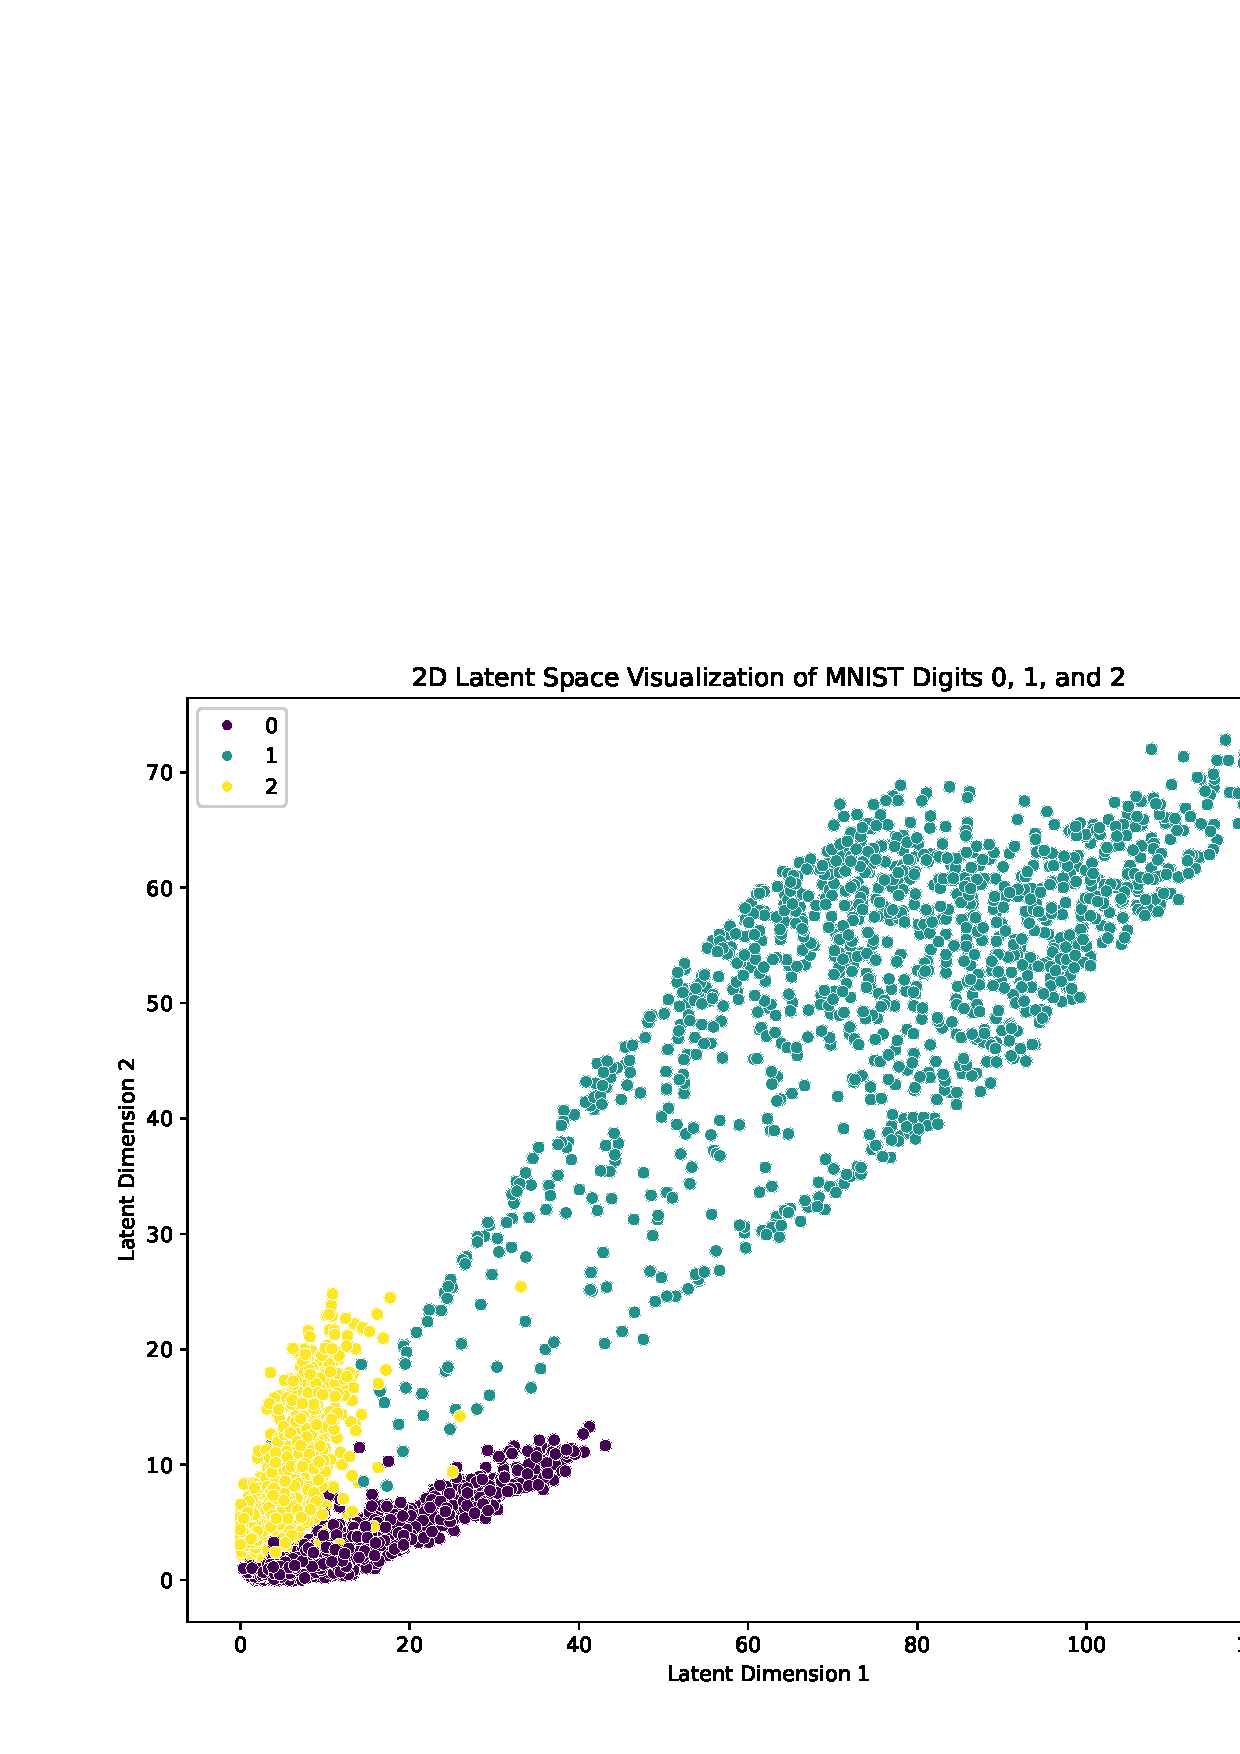
\includegraphics[width=7cm]{image-gen/picture/kaishi6.pdf}
\centering
\caption{MNISTデータセットの0、1、2の潜在空間における分布}
\end{figure}
\subsection{オートエンコーダーの生成}
一般に、画像生成では乱数を入力として処理を行い、画像を生成します。オートエンコーダーにおいては、潜在空間からランダムな値をサンプリングし、それをデコーダーに通すことで画像を生成します。

ここでは、図7の結果を基に、意図的に特定の手書き数字を生成できるかを検証します。ここで生成したい数字を「2」とすると、潜在空間内で「2」に対応するデータは、次元1が0から10、次元2が0から25の範囲内に分布しています。仮に、次元1の値を5、次元2の値を10とする潜在空間上の点を設定し、この点をデコーダーに通して画像を生成します。その結果、図8に示すように、手書き文字の「2」が生成されていることが確認できました。
\begin{figure}[h]
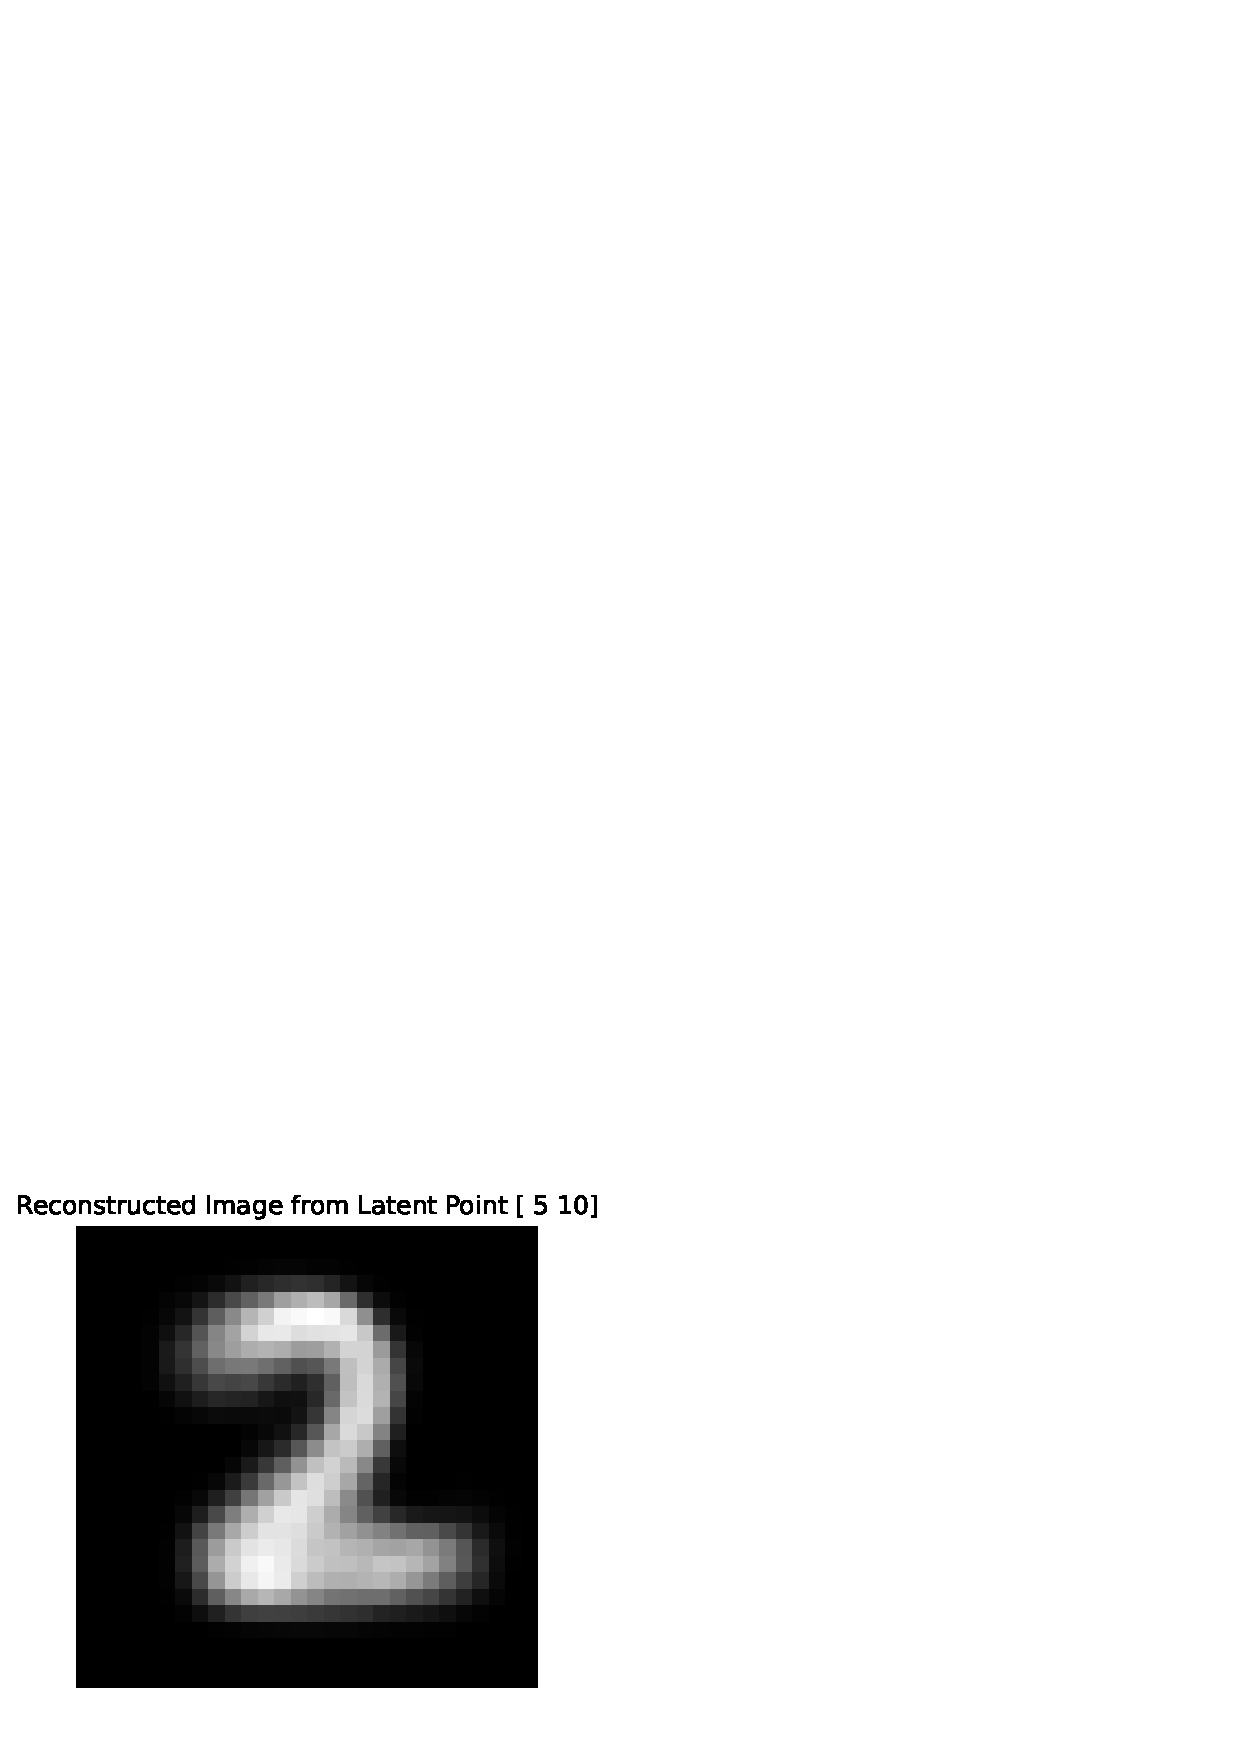
\includegraphics[width=7cm]{image-gen/picture/kaishi7.pdf}
\centering
\caption{潜在空間(5,10)の点から生成した画像}
\end{figure}
\section{ノイズ除去拡散モデル}
\subsection{ノイズ除去拡散モデルの概要}
この節からは、現在の画像生成技術の核となる拡散モデルについて解説します。拡散モデルは、2015年に機械学習および人工知能の研究者であるジャシャ・ソール=ディックスタインによって考案されたもので、非平衡熱力学の概念から着想を得ています。本節では、その中でも特に\textgt{ノイズ除去拡散モデル(Denoising Diffusion Probabilistic Models)}に焦点を当てて紹介します。

ノイズ除去拡散モデルの特徴は、オートエンコーダーのように一度の処理で画像を生成するのではなく、図9のように各ピクセルがランダムな値で構成された砂嵐(ノイズ画像)のような状態から、繰り返しノイズを除去する処理を行い、最終的に高品質な画像を生成する点にあります。
\begin{figure}[h]
\includegraphics[width=13cm]{image-gen/picture/kaishi8.pdf}
\centering
\caption{拡散モデルの画像生成過程例
出典:https://arxiv.org/pdf/2006.11239}
\end{figure}
\subsection{ノイズ除去拡散モデルの学習・画像生成}
まず、ノイズ除去拡散モデルを学習させるためのデータを作成します。ある画像に対して、段階的にわずかなノイズを加えていきます。この操作を繰り返すことで、最終的には各ピクセルが完全にランダムな値で構成された画像に近づいていきます。これは、図10における右から左への処理に対応します。これを\textgt{順方向の拡散過程}と呼びます。

この過程で得られる中間段階の画像と、それぞれの画像に加えられたノイズの情報を学習に利用します。学習の目的は、前述のとおり画像からノイズを除去することです。したがって、ノイズのある画像から加えられたノイズを予測し、その予測値を差し引くことで、ノイズを除去した画像を得ることができます。この処理は、図10における左から右への処理に対応し、画像にノイズを加える過程の逆操作を再現しているといえます。これを\textgt{逆方向の拡散過程}と呼びます。画像生成は、各ピクセルがランダムな値で構成された画像から始まり、前述のノイズ除去処理を繰り返すことで、最終的に高品質な画像が生成されます。
\begin{figure}[h]
\includegraphics[width=10cm]{image-gen/picture/kaishi9.pdf}
\centering
\caption{ノイズの付加と除去の過程 出典:https://arxiv.org/pdf/2006.11239}
\end{figure}
\subsection{ノイズ除去拡散モデルの構造}
それでは、画像に加えられたノイズをどのように予測するのかについて解説します。この問題をより一般的な観点から見ると、入力画像(ノイズを含む画像)と、予測すべき出力(ノイズ)が与えられていることになります。したがって、このタスクの構造は、オートエンコーダーにおける画像の圧縮と復元の過程に類似しています。

異なる点は、予測の対象がオートエンコーダーでは元の画像であるのに対し、ノイズ除去拡散モデルではノイズそのものであるという点です。したがって、基本的な構造はオートエンコーダーと同様に設計することが可能ですが、ノイズ除去拡散モデルでは、より高い精度を実現するために\textgt{U-Net}と呼ばれる構造が用いられます。

U-Netの構造は、オートエンコーダーと同様に、畳み込み処理によって特徴マップを圧縮するエンコーダーと、転置畳み込み処理によって特徴マップを拡大するデコーダーから構成されます。U-Net の特徴的な構造として、\textgt{残差接続}があります。
\begin{figure}[h]
\includegraphics[width=10cm]{image-gen/picture/kaishi10.pdf}
\centering
\caption{U-Netの構造 出典:https://arxiv.org/pdf/1505.04597}
\end{figure}

残差接続とは、図11に示すように、エンコーダー側の各段階で得られる特徴マップを、同じサイズのデコーダー側の特徴マップと積み重ね、その後、図4のように複数種類のフィルタを適用して畳み込み処理を行う構造です。この構造により、エンコーダーの途中で得られた空間的特徴情報がデコーダーに橋渡しされ、画像の位置関係などの情報を保持したまま、より高精度な予測が可能となります。
\section{潜在拡散モデル}
\subsection{潜在拡散モデルの概要}
この節では、イギリスの企業 Stability AI によって一般公開された画像生成モデル Stable Diffusion の中核となる\textgt{潜在拡散モデル(Latent Diffusion Model)}について解説します。Stable Diffusion は 2022 年 10 月に公開され、高価な専用機器を必要とせず一般的なパソコンでも実行できたことから、AI による画像生成が広く普及する契機となりました。

このモデルは、テキストによる指示に従って画像を生成する \textgt{text-to-image モデル}であり、現在一般的に想起される画像生成の代表的な形態です。Stable Diffusion は、ノイズ除去拡散モデルを基盤としつつ、さまざまな改良を加えることで、テキストの指示に忠実で高品質な画像生成を実現しています。

ここでは、その改良点のうち最も精度向上に寄与している\textgt{潜在拡散(Latent Diffusion)}について解説します。潜在拡散モデルでは、オートエンコーダーのように一度画像を圧縮して潜在空間を得た後、その潜在空間上でノイズ除去拡散モデルと同様のノイズ除去処理を行うことで、画像を生成します。
\subsection{潜在拡散モデルの構造・学習・生成}
以前のノイズ除去拡散モデルでは、画像の画素空間(ピクセル空間)上でノイズ除去を行っていたため、高解像度の画像を処理するには膨大な\textgt{計算量}が必要となります。ここでいう計算量とは、画像生成の際に必要となる加算や乗算などの演算回数を指します。計算量を削減しつつ、画像生成の表現力を両立している点が、潜在拡散モデルの大きな特徴です。

具体的には、まずオートエンコーダーと同様に、画像を圧縮および復元するように学習を行います。第3節で紹介したオートエンコーダーでは2次元に圧縮しましたが、潜在拡散モデルでは、より高次元である$32\times32$のような低解像度の特徴マップとして圧縮します。
\begin{figure}[h]
\includegraphics[width=13cm]{image-gen/picture/kaishi11.pdf}
\centering
\caption{潜在拡散モデル 画像:https://arxiv.org/pdf/2112.10752}
\end{figure}

図12に示すように、学習済みのオートエンコーダーに実際の画像を入力し、潜在空間上の特徴マップを得ます。この特徴マップに対して、ノイズ除去拡散モデルと同様に、段階的にノイズを加える処理(順方向の拡散過程)を行います。その後、ノイズが加えられた特徴マップからノイズを予測し、除去するように学習します(逆方向の拡散過程)。

最後に、画像を生成する際には、各ピクセルがランダムな値で構成された特徴マップから始め、前述のノイズ除去処理を繰り返した後、デコーダーを用いて最終的な画像を復元します。


\chapter{事前学習済みTransformerを用いた化学反応収率のベイズ最適化}\label{chap:bo-yield}
\section{はじめに}

ある日、あなたは研究室のボスから次のように言われました。  
「このリストの中から、最も収率のよい反応条件を探してくれ」と。

リストに載っている反応の数が10件程度であれば、すべてを試してみることも現実的かもしれません。  
しかし、それが数百件、数千件にも及ぶとなると話は別です。

化学反応には、温度・溶媒・触媒など、数多くの条件が関わります。  
それらの組み合わせをすべて網羅的に試すことは現実的ではありません。  
そのため研究者は、限られた実験回数の中で、見込みのありそうな条件や未知の可能性を秘めた条件を優先的に試す必要があります。

こうした「次にどの実験を行うべきか」を効率的に決定するための手法のひとつが、\textbf{ベイズ最適化(Bayesian Optimization)}です。

\section{ベイズ最適化とは}

機械学習に親しみのある方であれば、ベイズ最適化をハイパーパラメータチューニングの手法として耳にしたことがあるかもしれません。  
ベイズ最適化とは、\textbf{評価にコストがかかるブラックボックス関数を、できるだけ少ない試行で最適化する手法}です。

ブラックボックス関数とは、入力に対して出力を得ることはできるものの、その内部構造や関数形が不明な関数を指します。  
例えば化学反応の収率は、温度・溶媒・触媒など多様な条件に依存しますが、その関係は極めて複雑で、明示的な数式で表すことは困難です。

ベイズ最適化は、このようなブラックボックス関数の最適化において、少ない試行回数で最適解を探索するために用いられます。  
その流れは主に次の2つのステップから構成されます。

\begin{enumerate}
  \item \textbf{サロゲートモデルの構築}
  
  まず、既存のデータをもとにブラックボックス関数を近似する「サロゲートモデル」を構築します。  
  一般的には、\textbf{ガウス過程回帰(Gaussian Process Regression, GPR)}が用いられます。  
  GPRは入力空間における関数の振る舞いを確率的にモデル化し、予測値とその不確実性を同時に推定することが可能です。  
  予測値に加えて不確実性も考慮することで、未知領域を探索する指針を得ることができます。

  \item \textbf{獲得関数の最適化}
  
  次に、サロゲートモデルの予測結果をもとに「次にどの点を評価すべきか」を決定します。  
  その判断に用いられるのが\textbf{獲得関数(Acquisition Function)}です。  
  獲得関数は、予測値と不確実性の両方を考慮しながら、探索(exploration)と活用(exploitation)のバランスをとって次の候補点を選びます。  
  代表的な獲得関数には、\textbf{EI(Expected Improvement)}、\textbf{PI(Probability of Improvement)}、\textbf{UCB(Upper Confidence Bound)}などがあります。
\end{enumerate}

この2つのステップを繰り返すことで、ベイズ最適化は徐々に最適解に近づいていきます。  
特に、評価コストが高い場合や探索空間が広い場合において、その効率性が際立ちます。  
実験コストが高く探索空間が膨大な\textbf{化学反応条件の最適化}は、まさにベイズ最適化が最も有効に機能する領域の一つです。

\section{従来のベイズ最適化の課題}

ベイズ最適化は少ない試行で最適解を見つける強力な手法ですが、その性能はサロゲートモデルの精度に大きく依存します。  
一般的なベイズ最適化では、探索開始時にはデータが少なく、サロゲートモデルは初期のわずかなデータから構築されます。  

そのため、探索初期においては予測精度が低く、効率的な探索が難しいという問題があります。  
また、サロゲートモデルは通常、各タスクごとに一から学習を行うため、過去の実験データや他の反応系で得られた知識を活用できません。

一方、化学反応の分野には既に膨大な反応データや論文情報が存在します。  
にもかかわらず、従来のベイズ最適化ではそれらを活用せず、「毎回ゼロから探索を始める」という非効率な枠組みにとどまっています。

\section{事前学習済みモデルをサロゲートとして活用する}

従来のベイズ最適化では、サロゲートモデルは都度学習されるのが一般的です。  
しかし、近年の機械学習分野──特に自然言語処理や画像認識──では、\textbf{事前学習済みモデル(pretrained model)}の活用が標準的なアプローチとなっています。  
大規模データから汎用的な表現を学習し、それを個別タスクに転移することで、データが少ない段階から高い性能を発揮できることが知られています。

一方、ベイズ最適化の分野では、こうした「事前知識をもつサロゲートモデル」を導入した研究はまだ限られています。  
多くの手法は、対象ごとにデータを収集し、\textit{その場で一からモデルを構築する}という前提に立っており、  
初期段階では予測性能が十分でないのが現状です。

化学反応の最適化の文脈では、すでに多くの反応データベースや文献情報が整備されています。  
これらを活用しないのは大きな機会損失といえます。  
そこで本研究では、\textbf{事前学習済みの反応予測モデル}をベイズ最適化のサロゲートとして活用する手法を検討しました。

その一例として、今回はTransformerアーキテクチャに基づく収率予測モデルである\textbf{ReactionT5}\cite{sagawa2025reactiont5}を用いました。  
ReactionT5は約18万件の反応データを学習しており、化学反応の収率を高精度に予測する能力を持ちます。  
また、ファインチューニングにより特定の反応系に適応させることも可能です。  
これをサロゲートモデルとして利用することで、未知の反応条件に対しても初期段階から一定の予測精度を確保し、より効率的な条件探索が可能になります。

\section{ReactionT5を用いたベイズ最適化の枠組み}

全体の流れは図\ref{fig:bo_rt5}に示すように、従来のベイズ最適化と同様の構造を持ちます。  
ただし、ReactionT5のようなTransformerベースの事前学習済みモデルを含め、一般的なニューラルネットワークは推論時に確率的な振る舞いを持たないため、そのままでは不確実性の推定を行うことができません。したがって、これを可能にするためにはいくつかの工夫が必要となります。  
その中で最も簡単な手法の一つが、\textbf{MC Dropout}\cite{gal2015dropout}による不確実性推定です。

MC Dropoutでは、推論時にもDropoutを有効化し、複数回の推論を行うことで予測の分布を得ます。  
この分布の分散を不確実性の尺度として扱うことで、近似的にベイズ推定を実現します。  
Dropoutさえ含まれていれば、既存のニューラルネットワークに容易に導入できる点も利点です。  
本研究では、ReactionT5にMC Dropoutを適用して不確実性を推定し、ベイズ最適化のサロゲートモデルとして活用しています。

\begin{figure}[H]
  \centering
  \resizebox{\textwidth}{!}{
  \begin{tikzpicture}[
    node distance=14mm,
    box/.style = {draw, rounded corners, align=center, minimum width=32mm, minimum height=8mm},
    >={Latex[length=2.5mm]}
  ]
  \node[box] (model) {\shortstack{モデル\\\footnotesize(ReactionT5)}};
  \node[box, right=of model] (uncert) {\shortstack{不確実性推定\\\footnotesize(MC Dropout)}};
  \node[box, right=of uncert] (acq) {\shortstack{獲得関数最適化\\\footnotesize(EI / UCB / PI)}};
  \node[box, right=of acq] (exp) {\shortstack{実験・評価\\\footnotesize(新データ取得)}};
  \draw[->] (model) -- (uncert);
  \draw[->] (uncert) -- (acq);
  \draw[->] (acq) -- (exp);
  \draw[->] (exp.north) to[out=60, in=120]
    node[above, align=center, pos=0.5] {\footnotesize モデル更新\\{\footnotesize(学習/微調整)}}
    (model.north);
  \end{tikzpicture}
  }
  \caption{ReactionT5を用いたベイズ最適化の全体フロー}
  \label{fig:bo_rt5}
\end{figure}

\section{実験設計}
ベイズ最適化の有効性を評価するためには、未知の実験空間において、限られた試行回数で最適条件を効率的に探索できるかどうかを確認する必要があります。
そのため本研究では、ReactionT5の学習に使用されていない反応データセットを用いて検証を行いました。
具体的には、表\ref{tab:datasets}に示す3つのデータセットを使用しました。

Suzuki-MiyauraおよびBuchwald-Hartwigのデータセットについては、元のデータから「完全格子」と呼ばれる、すべての条件組み合わせが網羅された部分のみを抽出して利用しました。
これにより、探索空間が明確に定義された状態で、ベイズ最適化がどの程度効率的に高収率条件を見つけられるかを評価できるようにしました。
\begin{table}[H]
  \centering
  \caption{使用データセットと条件の組み合わせ}
  \label{tab:datasets}
  \begin{tabularx}{\textwidth}{@{}l X@{}}
    \toprule
    データセット名 & 組み合わせ \\
    \midrule
    NiB & \(33\) substrates \(\times\) \(23\) ligands \(\times\) \(2\) solvents \(= \num{1518}\) entries \\
    Suzuki-Miyaura
        & \(4\) reactant\_1 \(\times\) \(3\) reactant\_2 \(\times\) \(1\) catalyst
          \(\times\) \(11\) ligands \(\times\) \(7\) reagents \(\times\) \(4\) solvents
          \(= \num{3696}\) entries \\
    Buchwald-Hartwig
        & \(2\) ligands \(\times\) \(22\) additives \(\times\) \(3\) bases \(\times\) \(15\) aryl halides
          \(= \num{1980}\) entries \\
    \bottomrule
  \end{tabularx}
\end{table}

事前学習済みモデルとして、ReactionT5の収率予測モデルを使用しました。
このモデルに対してMC Dropoutを適用することで、予測値に加えてその不確実性も推定できるようにしました。
MC Dropoutの設定としては、ドロップアウト率をデフォルトの0.1に設定し、推論時に10回のサンプリングを行いました。

ファインチューニングは、探索を10回行うごとに実施し、それまでに得られた実験データを用いてモデルを更新しました。
得られたデータが25件以上となった場合には、学習データとテストデータを8:2の割合で分割し、テストデータにおける予測性能を確認しました。
ファインチューニングの設定は以下の通りです。

\begin{itemize}
  \item エポック数: 2
  \item 訓練バッチサイズ: 8
  \item 評価バッチサイズ: 16
  \item 学習率: \(1 \times 10^{-4}\)
  \item 最適化手法: AdamW
  \item Weight Decay: \(1 \times 10^{-2}\)
\end{itemize}
ベイズ最適化の獲得関数としては、Expected Improvement(EI)を採用しました。
通常のベイズ最適化では初期点をランダムに選択しますが、本研究では事前学習済みモデルを利用しているため、初期点もReactionT5の予測結果に基づいて選択しました。

また、比較対象として、OptunaのTPE(Tree-structured Parzen Estimator)Samplerを用いた手法と、RDKitから取得したMorgan Fingerprintを特徴量に用いたガウス過程回帰(GPR)ベースの手法を実装しました。

ベイズ最適化は確率的な手法であるため、それぞれの手法とデータセットに対して、シード値を変えて5回ずつ実験を行いました。

\section{結果}
NiB、Suzuki-Miyaura、およびBuchwald-Hartwigの各データセットに対するベイズ最適化の結果を図\ref{fig:results}に示します。
各グラフでは、横軸に試行回数、縦軸にこれまでに得られた最高収率をプロットしています。

\begin{figure}[H]
  \centering
  \includegraphics[width=\textwidth]{bo-yield/img/results.png} 
  \caption{各データセットにおけるベイズ最適化の結果}
  \label{fig:results}
\end{figure}

図\ref{fig:results}から、ReactionT5を用いたベイズ最適化が必ずしもすべてのデータセットで最良の性能を示すわけではないことがわかります。
NiBデータセットでは、ReactionT5ベースの手法は他の手法と比較して収束が遅く、最終的な最高収率も低い傾向を示しました。
一方、Suzuki-MiyauraおよびBuchwald-Hartwigデータセットにおいては、ReactionT5ベースの手法が他の手法を上回る性能を示し、より効率的に高収率条件を探索できていることが確認されます。

\section{考察}
図\ref{fig:results}の結果から、ReactionT5をサロゲートモデルとして用いたベイズ最適化は、従来手法と比較してデータセットによって挙動が異なることが確認されました。

まず、NiBデータセットにおいては、ReactionT5ベースの手法は他の手法に比べて収束が遅く、最終的な最高収率も低い傾向を示しました。
この要因として、NiBデータセットが他のデータセットに比べて化学構造や反応条件の多様性が高く、ReactionT5の事前学習時に十分に類似する反応が含まれていなかった可能性が考えられます。
すなわち、事前学習済みモデルに内在する「化学的事前知識」が、必ずしも未知の反応空間に対して有効に転移しない場合があることを示唆しています。

一方、Suzuki-MiyauraおよびBuchwald-Hartwigデータセットでは、ReactionT5ベースの手法がGPRベースおよびOptuna TPEを上回る性能を示しました。
これらのデータセットは、比較的均質な反応系から構成されており、事前学習済みモデルが学習している反応パターンと親和性が高かったと考えられます。
その結果、初期段階から高い予測精度を発揮し、少ない試行回数で高収率条件を見出すことができたと解釈できます。

総じて、本手法は「事前知識を有するサロゲートモデル」を導入することで、特定の反応系における探索効率を改善できる可能性を示しました。
一方で、NiBのように事前知識と対象系の分布が大きく異なる場合には、事前学習のバイアスが探索効率を損なうリスクもあるため、
モデルの適用範囲や、事前学習に用いるデータの選定方針が今後の課題として挙げられます。

\section{おわりに}
最後に、より大きな展望として「人間と道具」の関係について考えてみたいと思います。
この問題を考える上で外せない哲学者の一人に、ハイデガーがいます。
ハイデガーは、道具を含むあらゆる存在を「目的のために作られ、使われるもの」としての道具的連関から切り離し、
存在そのもののあり方として捉え直そうとしました。
この試みは、道具や自然を単なる客体的な利用の対象から解放し、
人間と世界との関わりそのものを見つめ直そうとするものでした。
しかしその過程で、人間と道具が協働し、「目的のために共に何かをなす」という、
本来あったはずの目的的な関係までもが、見えにくくなってしまったように思えます。

たとえば、職人にとっての道具は、単に同じ機能を備えていればよいというものではありません。
長年使い込まれた道具は、職人の身体の一部のように馴染み、
手の感覚や動きと一体化して初めて、最高の成果を発揮します。
そこには、単なる主体と客体の関係を超えた、相互に影響を及ぼし合う協働的な関係があります。
このように、人間と道具、さらには自然を含むあらゆる存在が互いに関わり合いながら、
共に目的を実現していく関係性を再構築することが、これからの科学技術にとって重要ではないでしょうか。

「事実から当為は導けない」というのは、広く共有された命題の一つです。
しかし、時として事実は、いかなる言葉よりも雄弁に当為を語り得ます。
もし、これからの科学技術研究に意義があるとするならば、それは実生活上の利益を超えて、
私たちが当然のものとして受け入れてきた主体と客体、人間と自然といった二項対立的な関係を問い直し、
新たな協働のあり方を模索することにあるのではないでしょうか。

本稿で取り上げたベイズ最適化のような手法や、あるいはAI技術全般が、
そのような新たな関係性の構築に寄与することを願っています。

今回の研究は、京都大学医学研究科・小島諒介先生のご指導のもとに実施しました。
本研究で使用した実験データおよびソースコードは、以下のGitHubリポジトリにて公開しています。

\begin{itemize}
  \item \url{https://github.com/kazumasa-okamoto/ReactionT5-bo-yield}
\end{itemize}


\chapter{Agenticな京大シラバス検索・時間割作成システム}\label{chap:syllabus}
\section{はじめに}

昨年度の11月祭では、我々は「完全一致のキーワード検索」にしか対応していなかった従来の公式シラバス検索システムに代わり、LLMによる文章埋め込み(Embedding)技術を用いて、ユーザーの検索意図をより深く反映した抽象的な検索を可能にするシラバスRAG(Retrieval-Augmented Generation)システムの開発に取り組んだ\cite{rag2021, internal2024rag}。本年度は、2023年以降に見られるAgent型AIの急速な発展を踏まえ、LLMを単なる情報検索の補助手段としてではなく、より能動的な「エージェント(Agent)」として活用することを目的とした。具体的には、ユーザーから提示される履修希望や興味・関心といった曖昧な要望を解釈し、時間割の空きコマや履修要件といった複雑な制約条件を考慮しながら、学期全体の時間割を自律的に構築・提案するシステムの開発を目指した。

\section{背景技術:プロンプティング手法とエージェント構造}
本プロジェクトで用いたLLMの制御手法として、基本となるプロンプティング手法であるCoT\cite{cot2023}から、外部ツール連携の基礎となるReAct\cite{react2023}、そしてPlan-and-Execute\cite{pande2023}のエージェント構造について順に解説する。
\subsection{CoT (Chain of Thought)}
Chain of Thought\cite{cot2023} は、大規模言語モデルに複雑な問題を解く際、最終的な答えに至るまでの推論過程を明示的に自然言語として生成させるプロンプティング手法である。単純な入出力のペアではなく、人間が問題を解く際の段階的な思考プロセスを模倣させることで、より正確で解釈可能な推論を実現する。
単に「Let’s think step by step(段階的に考えよう)」というフレーズを指示に加える(Zero-Shot-CoT)だけでも推論性能の向上が見られる。さらに、具体的な推論過程を例示するFew-Shot-CoTにより、Fine-tuningなどの追加学習を行うことなく、プロンプトの工夫のみで実装できる利点がある。

% \noindent % 行頭のインデントを避けるために置く(推奨)

\begin{minipage}[t]{0.48\textwidth}
\vspace{0pt}
    % --- 左側のボックス ---
    \begin{tcolorbox}[
        title=Standard Prompting,
        colback=white,
        colframe=gray,
        fonttitle=\bfseries
    ]
    
    \textbf{■ 質問:}
    カフェテリアには23個のリンゴがありました。昼食に20個使い、さらに6個買いました。リンゴは何個ありますか?
    
    \medskip
    \noindent
    \textbf{回答:} 答えは27個です。
    
    \end{tcolorbox}
\end{minipage}
\hfill % <-- 2つのボックスの間に空白を入れる
\begin{minipage}[t]{0.48\textwidth}
\vspace{0pt}
    % --- 右側のボックス ---
    \begin{tcolorbox}[
        title=Chain-of Thought Prompting,
        colback=white,
        colframe=gray,
        fonttitle=\bfseries
    ]
    
    \textbf{■ 質問:}
    カフェテリアには23個のリンゴがありました。昼食に20個使い、さらに6個買いました。リンゴは何個ありますか?
    回答は順序立ててステップごとに出力してください。
    
    \medskip
    \noindent
    \textbf{回答:}最初に23個ありました。20個使ったので、23-20=3個残りました。そして6個買ったので、3+6=9個になります。
    \end{tcolorbox}
\end{minipage}

CoTにより、算術推論・常識推論・論理推論など様々なタスクでの性能改善が見られた\cite{kojima2023}。さらに、CoTの性能改善はモデルの規模(スケール)に強く依存する「創発的性質(Emergent Abilities)」を示すことが知られている。一説には100B(1000億)パラメータを超えるような大規模モデルでは劇的な性能向上が観察される一方、それ未満のモデルでは標準的なプロンプティングと性能がほぼ同等に留まると報告されている。
CoTによってLLM内部の思考プロセスは改善され、推論能力は向上した。しかし、推論に用いる知識がLLM内部に事前学習されたものに限られるという課題(知識の陳腐化やハルシネーション)は依然として残る。

\subsection{ReAct (Reason and Act)}
前述のCoTが扱った「推論(Reasoning)」能力と、外部環境に対する「行動(Action)」を結びつけたものがReActフレームワーク\cite{react2023}である。
ReActは、LLMに「Reason(推論)」と「Act(行動)」を交互に生成させ、外部環境と相互作用しながらタスクを遂行するエージェントを実現する。ReActにおける「ツール(Tools)」は、LLMと外部環境を接続する重要なインターフェースとして機能し、「Act(行動)」によって引数付きで呼び出される。
ReActフレームワークは、以下の中核要素が循環的に相互作用することで動作する。

\begin{description}
    \item[(1)Thought(思考)]\leavevmode
        \begin{itemize}
            \item 現在の状況と利用可能な情報を分析
            \item 目標達成に向けて次に必要な行動を計画
            \item 過去の観察結果を統合して推論を更新
        \end{itemize}
    \item[(2)Action(行動)]\leavevmode
        \begin{itemize}
            \item 特定のツールを選択し、適切なパラメータで呼び出し
            \item 外部環境への具体的な操作を実行
            \item 情報取得や状態変更を実現
        \end{itemize}
    \item[(3)Observation(観察)]\leavevmode
        \begin{itemize}
            \item ツールの実行結果を受信
            \item 新たに得られた情報を文脈に統合
            \item 次の思考プロセスへのインプットとして機能
        \end{itemize}
\end{description}
ReActはCoTと同様に、追加のFine-tuningを必要とせず、few-shot promptingで実現される。

\begin{tcolorbox}[
    title=ReAct 応答例,
    colback=white, % ボックス内の背景色
    colframe=gray, % 枠線の色
    coltitle=white, % タイトルの文字色
    fonttitle=\bfseries % タイトルを太字に
    ]

\textbf{■ 利用可能なツール:}
\begin{description}
    \item[\texttt{Search[entity]}] Wikipedia APIを通じてエンティティ情報を検索
    \item[\texttt{Lookup[keyword]}] 現在参照中のページ内でキーワードを検索
    \item[\texttt{Finish[answer]}] 最終回答を出力してタスクを終了
\end{description}

\hrule % 水平線でセクションを区切る
\bigskip

\textbf{■ 質問:}
Apple Remote以外で、Apple Remoteが本来操作するように設計されていたプログラムを操作できる別のデバイスは何ですか?

\bigskip % 少しスペースを空ける

\textbf{■ 実行ログ (思考・行動・観察):}

\noindent % 段落のインデントをなしにする
\textbf{思考1:} Apple Remoteを調べて、それがどのプログラムを操作するように設計されていたかを知る必要がある。\\
\textbf{行動1:} \texttt{Search[Apple Remote]}\\
\textbf{観察1:} Apple Remoteは、2005年にAppleから発売されたリモコンで、Front Rowというメディアセンタープログラムを操作するために設計されていた。

\medskip % 小さなスペース

\noindent
\textbf{思考2:} Apple RemoteはFront Rowを操作するために設計されていた。次に、他にどのデバイスがFront Rowを操作できるかを調べる必要がある。\\
\textbf{行動2:} \texttt{Search[Front Row controls]}\\
\textbf{観察2:} Front Rowは、Apple RemoteまたはMacのキーボードで操作できる。

\medskip

\noindent
\textbf{思考3:} Front RowはApple RemoteとMacのキーボードで操作できることが分かった。\\
\textbf{答え:} \texttt{Finish[Macのキーボード]}

\end{tcolorbox}

\subsection{Plan-and-Execute}
ReActは強力なフレームワークである一方、いくつかの課題も存在する。ReActは「思考」と「行動」を密接に繰り返す(Thought-Action-Observationのループ)ため、局所的な最適解に陥りやすい。つまり、タスク全体を見通した大局的な戦略の維持が困難となり、長期的な文脈理解が必要なタスクでは元の目標を見失ったり、非効率なステップを繰り返したりする場合があった。

Plan-and-Execute\cite{pande2023}は、これらの課題に対処するため、役割を二つのLLM(あるいは二つの役割)に分離するアプローチである。

\begin{description}
    \item[Planner (計画者):]\leavevmode
        Executorが使用可能なツール群を前提として、与えられたタスクを達成するための一連の行動計画(サブタスクのリスト)を生成する。
    \item[Executor (実行者):]\leavevmode
        Plannerが生成した計画に基づき、各ステップを順次実行する。この際、ステップ内部ではReActのように思考とツールの使用を(局所的に)繰り返しながらサブタスクを遂行する。
\end{description}

\subsubsection{効果と性能改善}
Plan-and-Executeを採用する最大の利点は、認知負荷の分離にある。 複雑・長期的なタスクにおいて、Plannerは全体を俯瞰して計画を立案することに集中する。これにより、長期的な文脈の理解や冗長な行動の回避といった、大局的な最適化が可能になる。一方、Executorは計画全体を意識する必要がなく、目の前の局所的なサブタスク実行に集中できる。

もう一つの利点として、解釈可能性と介入可能性の向上が挙げられる。ReActが逐次的な思考の連鎖であるのに対し、本手法では最初に行動計画全体が明示されるため、システムが何をしようとしているのかを人間が容易に解釈できる。さらに、計画が生成された段階で人間がその内容をレビューし、修正を加えるといった介入も可能になる。

\section{データ設計と前処理}
京都大学が公開しているシラバスデータ\cite{kyodai2025syllabus}から、科目名・教員・成績評価・授業概要等の各種データを抽出し、検索に利用可能な状態へ前処理する基盤は、昨年度のRAGシステム開発の時点で確立していた。

本プロジェクトにおけるデータ処理は、この昨年度のデータを基盤としつつ、従来の「人間による検索」用から「LLMがツールとして利用」しやすい形式への変更、および「時間割全体の最適化」に必要な情報の追加を主眼とした。

データの前処理に関する詳細(基本的な抽出ロジック等)は昨年度会誌の記載\cite{internal2024rag}を参照されたい。本章では、昨年度からの主要な変更点と、エージェント化のために新たに追加した項目についてのみ詳述する。

\subsection{シラバスデータの変更点}
\subsubsection{メタデータ}
既存のシラバスデータから抽出したメタデータに対し、LLMが計算やフィルタリングに利用できるよう、以下の正規化と形式変更を行った。
\begin{itemize}
  \item 単位数\\
  従来「2単位」のような文字列型(str)であったデータを、エージェントが履修単位数を計算できるように数値型へ変更した。その際、「0.5単位」といった例外が存在するため、整数(int)型ではなく浮動小数点数(float)型を採用した。
  \item 開講年度・開講期\\
  「2025・前期」のように単一の文字列であったものを、「年度 (2025)」と「開講期 (前期)」の二つに分離し、メタデータ検索時の絞り込みを容易にした。
  \item 配当学年\\
  「全回生」「2回生以上」「主として1・2回生」など、表記揺れが多数存在したため、正規表現を用いてこれらを網羅的に解釈し、対象学年を示す数値のリスト(例: [1, 2])に正規化した。(薬学部等、6年制学部にも対応し1〜6の範囲とした。)
\end{itemize}
\subsubsection{シラバス本文}
シラバス本文は、そのままLLMに渡すには冗長であり、トークン長(コンテキスト長)とコストを圧迫する。そこで、LLMの認知負荷低減と情報圧縮の観点から、用途に応じて二段階の要約レベルを生成した。

1. 検索結果・授業比較用の構造化要約

これは、検索ツールがLLMに提示するための要約である。LLMが時間割に未登録の授業を評価・比較するために参照するものであり、授業の主要な情報は保持しつつ冗長性を排除する必要がある。 そこで、「授業のテーマ」「目的・背景」「主要トピック」といった項目をあらかじめ定義し、LLMに項目立てて構造化要約させた。これによりトークン数は平均で半分以下に抑えられた。また、副次的な効果として、情報の構造化によるLLMの認知負荷軽減も期待される。

2. 現在時間割の確認用・短縮要約

これは、既に時間割に組み込まれている授業の情報をLLMに渡す際に用いる要約である。他の授業との比較などを行わないため、詳細な説明は不要であり、キーワードや単文レベルまで情報を圧縮した。

\begin{tcolorbox}[
    title=検索結果の要約例,
    colback=white, % ボックス内の背景色
    colframe=gray, % 枠線の色
    coltitle=white, % タイトルの文字色
    fonttitle=\bfseries % タイトルを太字に
    ]
この授業で学べること
**中心テーマ:** 哲学史(古代から18世紀まで)
* **目的・背景:** 哲学の基本的な問いを理解し、古典的テクストを通じて哲学史的知識を身につけること。
* **主要トピック:** プラトン、アリストテレス、トマス・アクィナス、デカルト、ロック、カントの思想
* **得られるスキル:** 哲学的な問いを自ら考える能力、哲学史に関する基礎知識
\#\# 学習の進め方
* **授業スタイル:** 古典テクストの読解を通じた講義形式
* **学習の流れ:** 導入から始まり、各哲学者の古典を時系列で読み解く
\#\# 前提知識
* **推奨される知識:** 特になし
* **備考:** (授業内容からの推測)

\end{tcolorbox}

\begin{tcolorbox}[
    title=現在時間割用の要約例,
    colback=white, % ボックス内の背景色
    colframe=gray, % 枠線の色
    coltitle=white, % タイトルの文字色
    fonttitle=\bfseries % タイトルを太字に
    ]
哲学史の基礎/古代から18世紀までの主要哲学者の思想/古典的テクストの読解/哲学の基本的な問いの理解

\end{tcolorbox}


\subsection{単位取得率データ}
本プロジェクトでは、京都大学が公開している年度毎の「履修者数」と「単位取得者数」のデータ\cite{kyodai2025grade}を基に単位取得率を計算し、これを「単位取得の容易さ」を評価する指標の一つとしてLLMに提供した。
しかし、この単位取得率データには「科目名」と「開講部局」しか記載がなく、特に科目名は、一部が省略・変更されているため(例:「(演習)」やクラスコード「1S5」の欠落)、シラバスデータとの対応付けは困難であった。

今回は、特に楽単度合いの必要性が高いと想定される全学共通科目に絞り、以下の方法を用いてデータの紐付けを試みた。

\begin{enumerate}
  \item 正規化: 双方のデータに対し、半角全角の統一、空白文字の削除を行う。
  \item 前方一致検索: シラバスデータ側の授業名 S に対し、S.startswith(P) で完全にSに前方から含まれている単位取得率データ側の授業名 P を検索する。
  \item 最長一致の採択: S に対して複数の P が前方一致した場合(例:S="哲学II"に対しP1="哲学"とP2="哲学II"が一致)、最も一致文字列が長い P(この例では P2)を採択する。
  \item 開講部局による絞り込み: 上記で絞り込んでも複数の候補が残る場合、全学共通科目の開講部局である「国際高等教育院」のデータを優先する。
  \item データの合算: それでもなお候補が残る場合(例:学部生用と大学院用の同一名称科目)、データは区別せず、履修者数と単位取得者数を合算して扱った。
\end{enumerate}

この手法により、全学共通科目3154個の授業のうち、約95.6\%にあたる3015個のデータ紐付けに成功した。一方、残りの139個は対応するものが見つからなかった。 これら未対応データには、昨年度で廃講になった科目や、表記揺れの範疇を超えて名称変更された科目などが含まれると推測される。一部、名称が同一であるにも関わらず対応付けられなかったデータも存在し、これは今後の課題である。

\subsection{データ処理における課題}
現状のデータ前処理には、依然として多くの課題が残されている。

\begin{itemize}
  \item シラバスデータの形式が学部・学科毎に異なっており、現状では特定の学部(例:医学部)に一切対応できていないほか、他学部でも一部データの抽出ミスが散見される。
  \item 履修要件、クラス指定科目、推奨科目といった重要な制約条件の自動抽出が実現できていない。
  \item 単位取得率データは、全学共通科目以外(専門科目)には未対応。専門科目は科目名の揺れがより大きく、対応付けが格段に困難になるためである。
\end{itemize}

\section{時間割提案Agentの基本構造}
時間割提案Agentの基本的な機能について説明する。
\subsection{ユーザー情報の入力}
ユーザーの情報や要望についての入力について、チェックボックスやスライダーを用いて確実に入力できる構造化データの項目と、時間割全体への要望や興味関心のある分野などテキストベースで入力する項目の2つを用意した。
\subsubsection{確実に入力する構造化データ}
\begin{itemize}
  \item 学部・学科・学年
  \item 1限を許すか
  \item 空コマを許すか
  \item 全休を作りたいかどうか
  \item 授業を入れたくないコマ
  \item 授業形式への希望
  \item 授業評価方法の希望
  \item 既に履修することを決めている科目
\end{itemize}
\subsubsection{テキストによる入力}
テキスト入力欄を用い、主にユーザーの興味・関心分野や、上記項目では伝えきれない詳細な要望・制約を入力できるようにした。
初期実装では単一のテキスト入力のみであったが、後にLLMを用いて対話的に要求を引き出すチャット形式に変更した。ただし、この対話による要求抽出プロセスの高度化は、本プロジェクトでは十分に改良できず、今後の課題として残されている。

\subsection{LLMの利用ツール}
エージェントが環境(シラバスデータベースや内部の時間割状態)と相互作用し、タスクを遂行するために、以下の3つのツールを定義し、LLMがReAct形式で呼び出せるよう設計した。
\begin{itemize}
  \item 検索ツール \\
  シラバスデータベースから授業を検索する。基本的には昨年度と同様、FAISS\cite{faiss2017}を用いたシラバス本文のベクトル検索である。
  メタデータ検索では、複雑なand, or 検索まで可能ではあるが、初期実装ではLLMのツール利用を簡素化するため、検索パラメータを「曜日・時限」と「検索クエリ」のみに限定した。Plan-and-Executeアーキテクチャへの移行後は、Plannerの認知負荷が軽減されたため、任意パラメータとして「開講部局」「分野」「配当学年」等も指定可能とし、より高度な絞り込みを実現した。
  検索結果をToolMessageの形式で、「授業ID」「授業名」「曜日・時限」「授業形式」「評価方法」「単位取得率」「シラバス要約」をJSON形式で返す。
  該当する検索結果が見つからなかった場合は、ToolMessageで検索結果が見つからなかったことを返す。
  \item 授業追加ツール \\
  指定したIDの授業を現在の時間割に追加する。
  授業名による指定は、LLMの出力(表記揺れ)によって不安定となり、状態管理を複雑にするため、一意な授業IDを指定する形式を採用した。
  ToolMessageを用いて、授業の追加が成功したか否かを返す。失敗した場合は、その理由(「月曜2限が重複」等)も併せて返す。
  \item 終了ツール \\
  時間割提案完了・計画の各ステップのタスクの完了を判断した際に呼び出し、次のステップへと移行する。
\end{itemize}

\subsection{LLMへのデータ入力形式}
エージェントの思考ステップにおいて、プロンプトに含める現在の状態として、以下の情報を渡す。

具体的には以下のような形式で渡す。
\begin{tcolorbox}

\# 現在の状態\\
\#\# 現在の時間割情報\\
- **現在の時間割**:\\
月曜1限: 1227\\
月曜2限: 610\\
月曜3限: 無し\\
~~~\\
金曜5限: 無し\\
- **集中講義**: 無し\\
- **各授業idの詳細**:\\
1227: {'科目名': '英語リーディング ER30', '担当教員': ' 非常勤講師', '授業形式': ['演習'], '評価': {'平常点': 60, '課題': 0, '発表': 0, '討論': 0, '小レポート': 0,'小テスト': 0, '期末レポート': 40, '期末試験': 0}, 'シラバス本文': "アカデミックリーディングの基礎/学術入門書の精読/英語の学術的語彙/近代自然科学の歴史に関する知見"}\\
- **総取得単位数**: 21.0\\
- **学部**: 理学部\\
- **学科**: 理学科\\
- **現在の学年**: 1\\
\#\# ユーザーからの要望\\
- 一時限目には授業を入れないでください\\
- 一日の内で授業と授業の間に空いている時間があっても良い\\
- 授業が一つも入っていない曜日が作りたい\\
- 授業形式は、講義, 演習が好ましく、実験は避けたいです。\\
- 授業の評価方法は、講義, 演習が好ましく、実験は避けたいです。\\
- **避けたい曜日・時限**: 木曜5限\\
 **興味のある内容**: "1. **学びたい分野**:   - 数学系(特に応用的な分野) - 金融や保険数学  2. **興味のある応用先**:  - 金融  - 保険数学  - その他の数学の応用先(具体的には未記載) 3. **人文社会系の科目**:   - 経済  - 法律  - 社会に出てからも活躍しそうな内容.  **授業形式の希望**:   - 授業にあまり出たくない   - 期末レポートや期末テストの割合が高い形式を希望"

\end{tcolorbox}

\section{ReAct型Agent}
本プロジェクトの初期実装として、LLMが環境と相互作用しながら自律的にタスクを遂行するReActアーキテクチャ\cite{react2023}を採用した。将来的な一般公開時の運用コストを考慮し、LLMモデルには低コストな「gpt-4o-mini」を使用した。

\subsection{初期実装と課題}
初期の設計では、検索・授業追加・終了の3つのツールのみを用い、単一のLLMが「現在の状態(時間割情報)」と「ユーザー要望」に基づき、「思考」と「行動」を逐次的に繰り返す、シンプルなReActエージェントを構築した。

しかし、この構成で検証を行った結果、実用上、以下の深刻な問題点が多発した。
\begin{itemize}
  \item 探索の非効率性\\
  関連する授業が見つからない場合、LLMは同一または類似の検索クエリを際限なく発行し続け、検索の無限ループに陥る。
  \item 状態認識の欠如\\
  既に授業追加済みのコマを「空き」であると誤認し、重複して授業追加を試み、失敗する。エージェントはこの失敗から学習できず、同じコマへの追加を繰り返した。
  \item タスク完了判断不能\\
  時間割が十分に埋まった、あるいはこれ以上追加すべき授業がないという「タスク完了」の条件をLLM自ら判断できず、設定した最大ステップ数に達して強制終了するケースが多発した。
  \item トークン数制限\\
  ReActは設計上、過去の「思考・行動・観察」の全履歴をコンテキストに含める。これに加えて「現在の時間割詳細」という静的な情報も毎回のプロンプトに含めるため、思考が長くなると、APIのトークン数上限に容易に到達した。
\end{itemize}

\subsection{課題への対策}
上記の問題点を解決するために、次の2点を変更した。

一つ目は、プロンプトによる「空コマ」の明示である。時間割の情報から空いているコマを判断させてしまうとLLMの負荷が上がってしまうため、事前に空コマを求め明示的に与えることとした。これにより、既に埋まっている時間に授業を追加してしまう事だけでなく、検索の段階で埋まっている時間を検索してしまうという問題まで、大幅に削減できた。

二つ目は、思考履歴のトークン数による削減である。全履歴を渡す代わりに、トークン数で履歴を打ち切り、最新の思考のみをコンテキストに含めるよう変更した。この変更後も、エージェントのタスク遂行性能に顕著な低下は見られず、コストとAPI制限の問題を実用的なレベルで解決した。

\subsection{ReAct型の限界}
前節で述べた対策では根本的な問題は解決せず、システムプロンプトによって検索・授業追加・完了判断の思考方法について指示をしても、検索の失敗、不毛な授業追加の繰り返し、そしてタスク完了の判断ミスといった問題を本質的には解決できなかった。
また、ユーザーの興味関心のある授業を検索・追加することはできるが質が高いとは言えず、一般的な履修の決め方・履修要件などはほとんど考慮して考えることが出来なかった。
検証のため、gpt-5-miniなど少し上位のモデルを使用したところ、検索と授業追加に顕著な性能差が見られた。これによりタスクの成否がLLMの推論能力に強く依存することは確認できた。しかし、これにより我々は、本プロジェクトにおける最大のジレンマ、すなわち「性能とコストのトレードオフ」に直面することとなった。

低コストモデルでは、履修要件やユーザーの要望まで理解して検索・授業追加をすることが出来ず、高性能モデルでは要件を理解することはできるがReAct型の思考と行動の繰り返しにより、API料金が嵩んでしまう。
この「性能」と「コスト」のトレードオフは、ReAct型アーキテクチャを本タスクで実用化する上での根本的な障壁であると結論づけた。この問題を解決するため、我々はアーキテクチャそのものを見直し、「複雑な思考」と「単純な実行」を分離する必要があると考えた。これが、次章で述べるPlan-and-Executeアーキテクチャへの移行の直接的な動機である。

\section{Plan-and-Execute型Agent}
前章で述べたReAct型の根本的な課題、すなわち「性能」と「コスト」のトレードオフを克服するため、我々はPlan-and-Execute(計画・実行)アーキテクチャ\cite{pande2023}へと移行した。本アーキテクチャは、その構造的特性から、このジレンマに対する直接的な解決策となると判断したからである。

第一の利点は、LLMが担うべき認知的な負荷を分離することが出来る点にある。
\begin{itemize}
  \item Plannerは、履修要件、ユーザーの曖昧な要望、時間割全体のバランスといった、大局的で複雑なコンテキストの理解に集中する。
  \item Executorは、複雑な全体要件を考慮する必要がなく、Plannerから指示された個別のサブタスクの実行という、単純化されたタスクに集中できる。
\end{itemize}

第二の利点は、この役割分離により、役割に応じたLLMモデルの使い分けが可能となる点である。これは、ReAct型が直面した最大のジレンマに対する直接的な解決策となる。
\begin{itemize}
  \item Plannerは、複雑な要件を正確に解釈し、質の高い実行計画を立案するため、高性能・高コストなLLMを割り当てる。計画の立案はタスクの初回に一度だけ実行されるため、APIコストへの影響は最小限に抑えられる。
  \item Executorは、Plannerの計画に従ってツールを実行する(比較的単純な)役割であるため、低コストなLLMを割り当てる。Executorは「検索」や「追加」のたびに何度も呼び出されるが、安価なモデルを用いることで、全体のAPIコストを劇的に低減できる。
\end{itemize}

\subsection{Plan-and-Executor型の実装}
\subsubsection{Planner}
Plannerは、「ユーザー情報」「履修要件」「確定済みの授業」「推奨科目リスト」「履修戦略のヒント」といった情報をマークダウン形式で受け取り、実行計画を立案する。

特に、Plannerが複雑な思考に集中できる利点を活かし、LLMが単独では知り得ない情報(ドメイン知識)を参照情報としてプロンプトに組み込んだ。これはFew-Shotプロンプティングのように機能し、より質の高い計画を生成するよう出力を誘導した。

出力は、Executorが局所的な判断に陥らないよう、全体の方針を示す「全体の指針」と、具体的なサブタスクのリストである「計画」を含む厳格なJSON形式として定義した。

\subsubsection{Executor}
基本は今までのReAct型を原型としたが、役割に合わせて以下の点を変更した。
\begin{itemize}
  \item システムプロンプトで、全体の時間割を自律的に考えるための指示を削除し、Plannerの計画に従って検索・授業追加を行うように指示
  \item 従来のReAct型では、現在の時間割に加えユーザー情報などを毎回渡していた。しかし、Executorはユーザー情報を解釈する必要はないため、プロンプトから時間割以外の冗長な情報を削除した。各ステップの実行に必要な情報は、すべてPlannerが生成した計画から渡される。
\end{itemize}
\subsection{改善点}
ReAct型からPlan-and-Executeへ変更したことにより、生成される時間割の質が大幅に改善された。

第一に、本構成の主目的であったExecutorの動作安定性が向上した。ReAct型ではExecutor自身が思考する必要があったため、無駄な検索や失敗が多発していた。一方、本構成ではExecutorの役割が「計画の忠実な実行」に単純化された。Plannerから「検索クエリの方向性」や「授業の比較基準」が明確に与えられるため、よりユーザーの要望に沿った授業選択が可能となった。

第二に、時間割全体の質が向上した。Plannerが高性能モデルの推論能力を活かし、質の高い計画を立案できた場合に限定されるものの、その計画をExecutorが実行することで、人間が考案したものと遜色のないまともな時間割を提案できるケースも確認された。
しかし、この改善は、システム全体のボトルネックが「Executorの実行能力」から「Plannerの計画立案能力」へとシフトしたことを意味する。 LLMが本質的に知り得ない、各学部・学科固有の「ヒューリスティックな履修戦略」をPlannerに理解させ、質の高い計画を安定して生成させることは極めて困難であり、本稿執筆時点でもプロンプトの試行錯誤が続いている。

\section{今後の課題と展望}
本システムは現段階では未完成であり、多くの課題が残されている。
\begin{itemize}
  \item データ処理について、履修要件や推奨科目などまだまだ対応しきれていないものが多く残っている。
  \item 学部学科ごとに異なるようなヒューリスティックな履修戦略について、一部学部にしか対応できていない。
  \item LLMのコンテキスト理解とトークン数のバランスを取った時間割情報などの渡し方の試行錯誤。
  \item 計画の質が良ければ上手く時間割を考えられるが、Plannerの質の良い計画立案の制御がまだ完全にはできていない。
  \item Executorがタスクを完了できなかった際に、対応しきれず次のステップに移ってしまう。
  Executorで問題が起こった場合に、Plannerへ戻り全体を見通して計画の修正ができるようにしていく。
  \item 時間割を一度提案するだけでなく、提案した時間割をベースとしてユーザーとの対話しながら修正・改善できるようにする。
\end{itemize}

今回の11月祭までには、一般に公開できるレベルまでシステムの完成度を高めることはできなかった。 しかし、来春の新入生が入学する時期を目標とし、本章で挙げた課題の改善と試行錯誤を継続する。最終的には、より高精度かつ多機能な時間割提案エージェントとして公開できるよう、引き続き開発を行っていく。


\chapter{音楽と自然言語の類似度測定システムの開発}\label{chap:music-gen}
\section{はじめに}
\label{sec:introduction}
これまでの楽曲検索システムは曲名やアーティスト名、あるいはジャンルやテンポといったタグによる検索が主流でした。  
しかし、特定のタグやメタ情報だけでは「タグに存在しない感性的な要求」や楽曲の特徴からは直接推察できない要望に応えることが困難です。  
また、YouTube 等のプラットフォームでは話題性やランキングに基づいて検索結果が偏るため、純粋な類似性評価とは異なる順位付けが行われる場合があります。  
そこで本プロジェクトでは、自然言語クエリと音楽の類似度を直接測定するシステムを開発しました。
\section{アプリの機能}
\label{sec:features}
本システムは以下の主要機能を備えています。
\begin{itemize}
    \item \textbf{自然言語クエリ入力}:ユーザーは「激しい感情を歌った曲」や「リラックスできるメロディ」など、一般的な日本語表現で楽曲の特徴を指定できます。
    \item \textbf{CLAPモデルによる類似度測定}:CLAPモデルを用いて、テキストと音楽(音響特徴)間の類似度を計算します。
    \item \textbf{楽曲データベースとの照合}:事前に構築した楽曲データベース(J-POP中心)とクエリの埋め込みを比較し、類似度の高い楽曲を特定します。
    \item \textbf{類似度の可視化}:類似度に基づき楽曲をランキングし、2次元プロット等で可視化してユーザーに提示します。
\end{itemize}
これにより、ユーザーは従来のタグベース検索では見つけにくい、自身の意図に近い楽曲を効率的に探索できます。\\
\begin{figure}[h]
\begin{center}
\includegraphics[width=40mm]{music-gen/input.png}
\caption{クエリの入力例}
\end{center}
\end{figure}
\begin{figure}[h]
\begin{center}
\includegraphics[width=40mm]{music-gen/big_picture.png}
\caption{類似度の可視化結果}
\end{center}
\end{figure}
\section{推論・可視化の流れ}
\label{sec:inference_flow}
\subsection{概要}
ユーザーが自然言語で楽曲の特徴をクエリとして入力した際に、CLAPモデルを用いてテキストと音楽(音響特徴)の類似度を測定します。  
本節ではまず CLAP の基本構造と本研究での適用方針を説明し、その後で具体的な推論プロセスを示します。\\

\subsection{推論プロセス}
具体的な推論プロセスは以下の通りです。
\begin{enumerate}
    \item \textbf{クエリ入力と前処理}:ユーザーが「激しい感情を歌った曲」のような自然言語(日本語)クエリを入力します。
    \item \textbf{日本語から英語への翻訳}:Google Translation API を用いて英語に翻訳します。
    \item \textbf{テキスト・音楽埋め込みの生成}:翻訳したテキストとその他の多様なクエリ$X_s$を Text Encoder に、音源は前処理(メルスペクトログラム等)を行った上で Audio Encoder に入力し、埋め込みベクトル $E_{\text{query}}$ を生成します。
    \item \textbf{類似度の計算}:データベースに格納した楽曲の埋め込み $E_{\text{music},i}$ とクエリ埋め込み $E_{\text{query}}$ のコサイン類似度 $\mathrm{Sim}(E_{\text{music},i},E_{\text{query}})$ を計算し、各楽曲において、類似度スコアの平均で割ります。
    \item \textbf{検索結果の出力}:翻訳したテキストに関する類似度を基に楽曲をランキングし、類似度を座標軸として可視化してユーザーに提示します。
\end{enumerate}
この推論により、ユーザーは自身の意図した自然言語のニュアンスに近い楽曲群を探しやすくなります。\\
\subsection{CLAPモデルについて}
\label{subsec:clap}
CLAP\cite{elizalde2023clap}は、自然言語と音響を同一の埋め込み空間にマッピングすることを目的とした対照学習型モデルです。典型的には以下の構成を持ちます。
\begin{itemize}
  \item テキストエンコーダ(Text Encoder)とオーディオエンコーダ(Audio Encoder)を備えています。
  \item 対応するテキスト・音声ペアの埋め込みを近づけ、非対応ペアを遠ざける対照損失で学習します。
\end{itemize}
そのため、CLAP は「テキストで表現された音の概念」と「実際の音響特徴」を意味的に結びつけることができます。ゼロショット検索やテキスト条件付きの音検出に有効であり、本研究ではこれを日本語クエリと楽曲の類似度測定に応用します。\\
既存の CLAP は環境音や一般音声を中心に学習されていることが多く、楽曲固有のメロディや楽器、ハーモニーといった特徴を扱うには、対象ドメイン(例:J-POP)でのファインチューニングが有効です。そこで本研究では CLAP の Text/Audio Encoder を J-POP データで微調整し、日本語クエリに対して高精度な類似度評価が行えるように設計します。\\
\begin{figure}[h]
\begin{center}
\includegraphics[width=60mm]{music-gen/clap.png}
\caption{可視化結果}
\end{center}
\end{figure}
\section{学習の流れ}
\label{sec:training_flow}
\subsection{概要}
既存の CLAP モデル(例:laion/clap-htsat-fused)はクラシックや環境音中心に学習されているため、日本の楽曲に対する類似度測定には最適化されていません。  
本研究では J-POP を中心としたデータセットで CLAP をファインチューニングし、日本語クエリと楽曲埋め込みの対応を強化します。\\

\begin{enumerate}
 \item \textbf{データセットの構築}:日本の楽曲を対象に、楽曲ファイル(オーディオ)と対応するテキストデータ(YouTube コメント、歌詞、タグ等)を収集します。
 \item \textbf{ノイズ除去}:収集したテキストデータにはノイズが含まれるため、フィルタリングや前処理で不要な情報を除去します。
 \item \textbf{対照学習}:正例ペア(対応する楽曲とテキスト)間の類似度を最大化するように対照損失で学習します。
\end{enumerate}
この手順により CLAP は日本語の表現と楽曲の音響特徴との対応関係を深め、実用的な類似度評価が可能になります。\\
\subsection{データセットの構築}
学習用に使うデータセットとして必要なのは、プレビュー音源(オーディオ)、歌詞、タグ、曲の感想を表すコメントやレビューの情報(テキスト)です。\\
プレビュー音源(30秒)については、アーティスト名のリストを手動で作成し、それらをITunes Search APIによって検索をすることで取得します。各アーティストにつき上位5曲を検索します。曲の人気度や新しさなどに基づいて検索される曲が選ばれています。これにより、同時に曲のトラック情報やメタ情報を取得することができます。\\
歌詞については、Genius APIを用いてアーティスト名、曲のタイトル名で検索し、取得できる部分は取得します。Genius APIの検索で辿り着かない一部楽曲はmusic.jpというWebサイトをWebスクレイピングすることにより、取得します。以上の方法により楽曲の情報が取得できた楽曲を対象に、学習を行います。\\
楽曲の特徴や感想を表すコメントやレビューの情報の収集については、YouTube Data APIを用います。該当する楽曲のMVをアーティスト名、曲のタイトル名で検索し、そのコメント欄から各曲100件ずつ収集します。コメントは新しい順、人気順の二つのソートの方法がありますが、良質なコメントを多く集めたいので、人気順を選択しました。Youtubeのコメント欄は学習に有用な、曲の特徴を表したコメントばかりではありません。学習に不向きなコメントは次に解説する手順で除去することで、CLAP側のファインチューニングの精度の向上を試みました。\\
\subsection{ノイズとなるコメントの除去}
日本語版BERT\cite{sawada2024release}\cite{rinna-japanese-roberta-base}を用いてコメントを以下のラベルに分類し、ラベル0に該当するコメントのみ曲の特徴を表していると判断して残すことにしました。今回用いたモデルはRoBERTaをベースにしたものです。RoBERTaはNSP(次の文章の予測タスク)を削除したり、マスキングパターンを固定しないなど、BERTの学習手法をロバストに最適化されています。このモデルは今回のような分類タスクに優れています。\\
\begin{enumerate}
  \item \textbf{ラベル0}:曲の感想や、曲にまつわる投稿者のエピソード(例:儚いラブソングだと感じました。)
  \item \textbf{ラベル1}:曲に関連するMVやアニメ、ドラマなど、関連コンテンツに関するコメント(例:昨日のドラマはとてもよかった)
  \item \textbf{ラベル2}:曲の再生数や人気度に関するコメント(例:祝1億回再生!)
  \item \textbf{ラベル3}:アーティストのビジュアルや行動、エピソードに関するコメント(例:ドラマの主題歌書かせたらこの人がピカイチだね)
  \item \textbf{ラベル4}:曲に関係ない、雑多なコメント(例:毎日〇〇日記)
  \item \textbf{ラベル5}:歌詞
\end{enumerate}
BERTのファインチューニングには事前に教師データを用意しておく必要があります。教師データのラベリングについては手動で600件行いました。ラベル0や4が多くなり、ラベル5は少ないなど、ラベルの不均衡が起きていたため、少ないラベルに該当するデータをコピーして水増ししました。これによって、データが1200件まで増え、全てのラベルに属するデータを均等に学習することができます。\\
学習時では91%の正解率(accuracy)でラベル分類が行われました。全部のデータに手動で正解ラベルを与えたわけではないため、実際のコメントのラベル分類の正解率は正確には分かりませんが、これと同等の精度で分類できていると期待できます。実際、歌詞コメントなど、曲の内容に無関係なコメントは除去できていました。\\

\subsection{対照学習の方法}
\label{sec:contrastive_method}
本システムでは、\textbf{正例ペアのみを収集したデータセット}を用い、\textbf{InfoNCE Loss}に基づく対照学習を実行することで、モデルにオーディオとテキストの対応関係を学習させます。

\begin{enumerate}
    \item \textbf{日本語テキストの英訳と埋め込み}:
    CLAPモデルの事前学習を考慮し、収集した\textbf{日本語テキスト}は、学習前に\textbf{Google Translation API}を用いて英語に機械翻訳します。これにより、翻訳された英語テキスト $T$ と対応する楽曲データ $A$ のペア $(A, T)$ が学習の正例として用いられます。これらはそれぞれAudio EncoderとText Encoderに入力され、埋め込みベクトル $\boldsymbol{v}_A$ と $\boldsymbol{v}_T$ に変換されます。

    \item \textbf{損失関数 InfoNCE Loss の基盤}:
    損失関数には、バッチ内ネガティブサンプリング(In-batch Negative Sampling)の特性を持つ\textbf{InfoNCE Loss}(Information Noise-Contrastive Estimation Loss)を用います。この手法は、データセットから負例を明示的に用意しなくても、学習に利用されたミニバッチ内の正例でない組み合わせを自動的に負例として扱う仕組みです。

    具体的には、ミニバッチ内に $N$ 個の正例ペア $\{ (A_1, T_1), \dots, (A_N, T_N) \}$ があるとき、オーディオ $A_i$ に対するテキスト $T_i$ は\textbf{正例}ですが、それ以外のテキスト $T_j$ ($j \neq i$) は全て負例として機能します。これにより、$N$ 個の正例と $N(N-1)$ 個の負例が損失計算の過程で暗黙的に機能します。

    \item \textbf{対照損失の計算とモデルの学習}:
    InfoNCE Loss $\mathcal{L}_{A \to T}$ は、オーディオ埋め込み $\boldsymbol{v}_{A, i}$ が、バッチ内の $N$ 個のテキスト埋め込みの中から、正解テキスト $\boldsymbol{v}_{T, i}$ を正しく識別できる確率を最大化するように定義されます。コサイン類似度 $\text{sim}(\boldsymbol{v}_{A, i}, \boldsymbol{v}_{T, j})$ を用いた、オーディオ $A_i$ に基づく損失 $\mathcal{L}_{A \to T, i}$ は以下の通りです。
    \begin{align}
        \mathcal{L}_{A \to T, i} &= - \log \frac{\exp(\text{sim}(\boldsymbol{v}_{A, i}, \boldsymbol{v}_{T, i}) )}{\sum_{j=1}^{N} \exp(\text{sim}(\boldsymbol{v}_{A, i}, \boldsymbol{v}_{T, j}) )}
    \end{align}

    最終的な対照損失 $\mathcal{L}$は、オーディオからテキストへの損失 $\mathcal{L}_{A \to T}$ と、その逆 $\mathcal{L}_{T \to A}$ の双方向の和として計算され、これを最小化することで学習を行います。

    $\mathcal{L} = 0.5×\frac{1}{N}\sum_{i=1}^{N} (\mathcal{L}_{A \to T, i} + \mathcal{L}_{T \to A, i})$

    学習の目的は、正例ペア間の類似度を最大化し、負例として機能するバッチ内の非対応ペア間の類似度を最小化することで、エンコーダが楽曲の音響特徴と英訳されたテキスト表現の間の対応関係を学習することです。
\end{enumerate}
この手法でCLAPモデルをファインチューニングすることで、日本語クエリと楽曲の類似度測定に特化した性能向上がされました。\\
実際に学習後のモデルを用いて、自然言語クエリと楽曲の類似度測定を行った結果、ユーザーの意図に近い楽曲が学習前の時より上位にランクインするなど、実用的な性能が確認された。\\
\begin{table}[h]
\caption{「力強く歌うことで、葛藤から克服しようとしている」というクエリに対する類似度評価の比較}
\begin{center}
\begin{tabular}[t]{|c|c|c|}
\hline
\diagbox{楽曲}{モデル} & $変更前$ & $変更後$ \\
\hline
 残響賛歌  & $-0.9784$  & $0.9528$ \\
\hline
 天体観測  & $1.1011$ & $0.9412$ \\
\hline
 群青 & $-0.9766$ & $0.9510$ \\ 
\hline
\end{tabular}
\end{center}
\end{table}
\section{おわりに}
\label{sec:conclusion-music}
本研究では、自然言語クエリと楽曲オーディオを同一埋め込み空間で比較するシステムを提案しました。  
ユーザーは感性的な日本語表現を用いるだけで、自身の意図に近い楽曲を効率的に探索・可視化できます。  
しかし、「米津玄師みたいな曲」のような固有名詞を伴うクエリに対しては、CLAP の事前学習データに依存するため、十分な類似度評価が難しいため今後の課題となります。
今後はこういった面も含めて、CLAP のさらなる最適化、多ジャンル対応を行うことでより広範なユーザー体験の向上を目指します。



\chapter{顔認識で操作するゲーム}\label{chap:face-game}
\section{はじめに}
「目は口ほどに物を言う」という言葉が示すように、人間同士のコミュニケーションにおいて表情はきわめて大きな役割を担っています。しかし現在のヒューマン–コンピュータ・インタラクションにおいては、そのモダリティの多様性にもかかわらず、依然としてキーボード入力や音声指示といった言語的・運動的な情報に強く依存したままです。

もしこの制約を超え、表情そのものを操作インタフェースとして利用できれば、より自然で直感的な応答が可能となります。そこで本プロジェクトでは、顔表情認識を用いて操作するゲームを開発し、表情入力のユーザビリティと可能性を検証することを目的とします。

\section{使用ライブラリ・論文解説}
本プロジェクトでは、顔認識の基盤として Google が提供するMediaPipe Face Landmarker\cite{mediapipe_face_landmarker_2024} を採用しています。MediaPipe Face Landmarker は、顔の目や口といった主要ランドマークをCPU 環境でもリアルタイムに推定できる軽量・高精度なライブラリであり、表情入力を扱う本プロジェクトに非常に適しています。

このライブラリを利用することで、ユーザーの細かな表情変化を高い精度・低遅延で取得でき、自然かつ滑らかな操作体験を実現できる点が大きな利点です。

MediaPipe Face Landmarker は、Google が開発した軽量顔検出器 BlazeFace\cite{bazarevsky2019blazeface} を基盤として構築されています。本節は、その論文をもとに、その主要なアーキテクチャ上の特徴を概説します。

BlazeFace は、モバイル GPU 上での推論に特化して設計された軽量かつ高速な顔検出モデルです。スマートフォン上で 200–1000 FPS という極めて高い速度で動作し、AR アプリケーションなどで求められる 2D/3D ランドマーク推定や表情分類へほぼ遅延なく顔領域を提供できる点が特長です。

この革新的な性能は、以下の三つの主要なアーキテクチャ上の工夫によって実現されています。

\subsection{軽量な特徴抽出ネットワーク}
MobileNetV1/V2\cite{howard2017mobilenets}\cite{sandler2018mobilenetv2}に着想を得ながらも、モバイルでの物体検出に最適化された独自のコンパクトなネットワークを採用しています。このネットワークでは、図\ref{fig:blazeface_architecture}に示すように、一般的な3x3カーネルの代わりに5x5カーネルを用いた深度方向分離可能畳み込み(depthwise separable convolution)をモデルのボトルネック部分で活用します。これにより、演算量を抑えつつも、より少ない層で広い受容野(receptive field)を確保し、効率的な特徴抽出を可能にしています。 

\begin{figure}[H]
    \centering
    \includegraphics[width=0.6\textwidth]{face-game/img/blazeface_architecture.png}
    \caption{BBlazeBlock(左)とダブルBlazeBlock(右)のアーキテクチャ}
    \label{fig:blazeface_architecture}
\end{figure}

\subsection{GPUに最適化されたアンカー方式}
BlazeFaceでは、GPUの処理特性に合わせた独自のアンカー生成方式が採用されています。一般的なモデルが特徴マップを1×1まで段階的に縮小していくのに対し、BlazeFaceは図\ref{fig:blazeface_anchors}に示すように解像度を8×8で止め、それ以上のダウンサンプリングを行いません。

これは、低解像度の特徴マップを扱う際に発生する GPUディスパッチの固定オーバーヘッドを削減し、推論速度の大幅な向上につながる設計です。

\begin{figure}[H]
    \centering
    \includegraphics[width=0.8\textwidth]{face-game/img/blazeface_anchors.png}
    \caption{BlazeFaceのアンカー方式}
    \label{fig:blazeface_anchors}
\end{figure}

\subsection{後処理でのtie resolution戦略}
物体検出では多くの場合、複数のバウンディングボックスの候補が同一の物体を指す場合にNMS(Non-Maximum Suppression)を用いて1つのバウンディングボックスに絞り込みますが、BlazeFaceはNMSに代えて 独自のブレンディング戦略を採用しています。

複数のバウンディングボックスの重み付き平均を取ることで最終出力を決定し、フレーム間での検出結果のちらつき(時間的ジッター)を大幅に低減します。その結果、より滑らかで安定した検出が実現されます。

\subsection{まとめ}
これらの工夫により BlazeFace は、モバイル環境における顔検出の速度と精度の基準を大きく引き上げました。そしてその成果は MediaPipe Face Landmarkerを通じて、現在の多くの AR・表情認識アプリケーションの基盤技術となっています。

\section{ゲーム入力の実装}
本節では、MediaPipe ライブラリを用いた表情認識によるゲーム入力の実装について、主に工夫した箇所に絞って解説していきます。

\subsection{入力の詳細}
今回はリアルタイム推論を行うので、比較的検出しやすい「まばたきをする」「口を開ける」「笑顔になる」の3つの表情入力を対象とします。各表情は立ち上がり時(しきい値を下回る状態から上回った瞬間)に一度だけ入力として扱います。長押しのような操作は存在しません。

\subsection{軽量化・遅延削減}
今回の実装において、肝となるのはやはり軽量化・遅延削減です。ゲーム入力にはリアルタイム性が求められるため、表情認識をいかに素早く処理してゲームに反映させるかが重要になってきます。最適化を行わなかった初期実装では、ゲーム画面がカクついて到底快適ではありませんでした。画面にカクつきが生じるのは、1フレーム当たりの推論時間が描画間隔に対して間に合っていなかったのが原因であると考えられます。そこで実装したのが非同期推論です。

非同期推論とは、ゲームの描画とは別の時間軸で表情認識の推論を行う機能です。初期実装では、1フレームの推論が完了してから次のフレームの描画を始めていました。対して非同期推論では、1フレームの推論の進捗に関わらず、次のフレーム描画を始めます。安定したフレームレートが重視されるゲーム描画には、この非同期推論は有効でしょう。表情認識処理とは無関係に描画が行われるので、画面のカクつきはこれで解消することができます

では実際、どのように非同期推論を実装しているのかについても少し触れておきます。

MediaPipe Face Landmarkerには、標準機能で非同期推論を行うLIVE STREAMモードが搭載されています。今回の場合では、メインの描画処理とは別スレッドで、このLIVE STREAMモードで表情認識処理を行い、その処理結果を入力として採用しています。

さて、非同期推論を導入したことで画面のカクつきは解消されました。しかし、このままではもうひとつ問題があります。表情認識処理が非同期になった分、入力の遅延が発生してしまったのです。以前までの同期推論では、表情認識処理が完全に終了してから次のフレームが描画されるため、遅延の問題は発生しませんでした。そこで、次は推論自体を軽量化することで、遅延の解消に取り組みます。

具体的には、解像度の縮小とフレームレートの削減を行っています。表情認識処理に入力する画像の解像度を下げることで、処理は軽量になりますが、そのぶん精度の低下にもつながります。しかし、今回は「口を開ける」「まばたきをする」「笑顔になる」という比較的検出しやすい3つの特徴を区別できればよく、解像度を80×60ピクセル(幅×高さ)まで下げてもプレイにはあまり問題は生じませんでした。同様にフレームレートに関しても、60fpsから15fpsまで下げることで軽量化と精度の維持を両立しています。

加えて、カメラのバッファサイズの削減、MJPEG の使用、CPU/GPU デリゲートの切り替えにも対応しました。これらにより、入力タイミングの精度が求められるrunnerゲームにおいても、遅延を気にせず快適にプレイできる水準を実現しました。

\subsection{検知精度の向上}
先ほどまでは軽量化・遅延削減の工夫を解説してきましたが、次に表情入力検知について紹介します。「まばたきをする」「口を開ける」「笑顔になる」の3入力それぞれに関して、検知条件などを解説していきます。

まず、「まばたき」の検出に関しては、右目と左目における「まばたきの程度(eyeBlink)」の平均値に加えて、補助的に「目の細め具合(eyeSquint)」の平均値も用いています。これらの平均値のうち最大値を使用することで比較的高精度で「まばたき」を検出することができました。

次に、「口を開ける」の検出には「あごの開き具合(jawOpen)」と「口の開き具合(1 - mouthClose)」の二つを用いています。「あごの開き具合(jawOpen)」は数値が出ないことがあったので、予備の条件として「口の開き具合(1 - mouthClose)」を使用しています。

最後に、「笑顔」の検出には「左右の口角の上がり具合(mouthSmileLeft/Right)」を用いたうえで、予備の条件として、「左右の口角の引き上げ量(mouthCornerPullLeft/Right)」も用いています。残念ながら口角を動かさずに笑う人の笑顔は検出できなさそうですね。

これらに加え、検出のON/OFF に異なるしきい値を設けるヒステリシスにより、誤検知やチャタリングを抑制しています。

\section{制作ゲームの紹介}
表情認識を用いて制作したゲームのうち、代表的な2作を紹介します。

\subsection{Runner}
当研究会のマスコットキャラクター「KaiRA 君」を操作し、迫り来る障害物を避ける横スクロールアクション。「口を開ける」とジャンプし、タイミングよく障害物を回避します。どこか某ブラウザの恐竜ゲームを想起させる内容です。

\begin{figure}[H]
    \centering
    \includegraphics[width=0.6\textwidth]{face-game/img/runner_game.png}
    \caption{runnerゲームのプレイ画面}
    \label{fig:runner_game}
\end{figure}

\subsection{Speed React}
次々と提示される状況に対して、素早く正確なリアクションを求められる独創的なゲーム(バカゲー)。「笑顔」「驚いた顔」「真顔」のうち状況に合ったリアクションを行います。2人対戦が可能な「VS React」も用意しています。

\begin{figure}[H]
    \centering
    \includegraphics[width=0.6\textwidth]{face-game/img/speed_react_game.png}
    \caption{Speed Reactゲームのプレイ画面}
    \label{fig:speed_react_game}
\end{figure}

\section{おわりに}
本プロジェクトでは、表情認識を用いたゲーム操作を通じて、人間とコンピュータの新しい関わり方の可能性を検討しました。実装を進めるなかで強く感じたのは、表情を入力として扱うことは想像以上に難しいという点です。その理由のひとつは、表情がしばしば意図的な操作ではなく、無意識の反応として現れる情報だからです。

キーボードやマウスのような明確な「命令」とは異なり、表情は感情や注意の変化、緊張や驚きといった非言語的で曖昧な状態をそのまま映し出します。したがって、表情をインタフェースとして用いることは、単なる操作系の設計を超えて、人間の身体性や無意識との向き合い方を考える営みでもあると感じました。

しかし同時に、もし将来「無意識のコンピューティング」とでも呼べるような新しいインタラクションの枠組みが成立するとすれば、そのもっとも素朴で原初的な入口は、表情によるインプットなのかもしれません。意図と言語を介さず、身体が自然に発する信号をそのまま拾い上げることができる点で、表情は人間の奥深いレイヤーに最も近い情報だからです。

今回の試みは小さな実装にすぎませんが、ヒューマン–コンピュータ・インタラクションがより「人間そのもの」に寄り添う方向へ進む可能性を垣間見ることができました。今後は、表情だけでなく姿勢や視線、呼吸などのマルチモーダルな信号を統合することで、より自然で直感的なインタラクションが実現できると考えています。本プロジェクトがその一歩となれば幸いです。


\chapter{歩くKaiRA君:強化学習を用いた二足歩行ロボットの歩行制御}\label{chap:rl-kaira}
\section{はじめに}
\label{sec:intro}
近年、強化学習によってロボットの自律的な動作が可能になりつつあります。\\
特にロボット分野では、学習したダイナミクスで接触遷移や外乱を見越し、凹凸路や滑り面での歩行・バランス回復を組み立てるといった事例が増えています。
そして、それを応用して災害時の救助用ロボットが開発されたりしております。\\
そこで今回は、強化学習による、KaiRAくんの2足歩行を図る手法—シミュレータ学習について解説します。
% --- 第2章 ---
\section{学習目標}
\label{sec:target}
本プロジェクトでは、Unity ML-Agentsを用いて、二足歩行ロボット(KaiRAくん)をシミュレーション環境で学習させる。\\
学習環境には目標オブジェクトが存在し、図1の矢印の方向に置かれている。\\
KaiRAくんは、4つの関節(左右の上脚・下脚)を持ち、できるだけ早く目標に向かって歩行することを目的とする。\\
この目的を達成するために、観測情報を基に行動(関節の目標回転角と駆動強度)を決定し、報酬関数とPPO\cite{schulman2017proximal}を用いて学習を進める。\\
\begin{figure}[h]
\begin{center}
\includegraphics[width=50mm]{rl-kaira/overview.png}
\caption{KaiRAくんの概観}
\end{center}
\end{figure}
\\
% --- 第3章 ---
\section{学習フロー}
\label{sec:foundation}
本節では、二足歩行ロボット(KaiRAくん)をシミュレーション環境で学習させるための具体的な構成と、学習を導くための報酬設計について述べる。
学習フローは以下の通りである。\\
\begin{enumerate}
    \item \textbf{観測(Observations)}:エージェント(KaiRAくん)は、環境と自身の状態に関する情報を観測する。
    \item \textbf{行動(Actions)}:観測情報に基づいて、行動方策(ニューラルネットワーク)によってエージェントの関節の目標回転角と駆動強度を決定する。
    \item \textbf{環境への適用}:決定された行動が物理エンジンに適用され、KaiRAくんの動作がシミュレーションされる。
    \item \textbf{報酬の取得(Reward)}:目標に向かって歩行する度合いに基づいて報酬を受け取る。
    \item \textbf{学習の更新}:収集された観測、行動、報酬のデータを用いて、エージェントの行動方策がPPOによって更新される。
\end{enumerate}

\subsection{観測}
エージェントは、環境と自身の状態に関する合計24次元の情報を観測し、これをニューラルネットワークへの入力とする。\\
\begin{itemize}
  \item \textbf{目標との関係(11次元)}:
    \begin{itemize}
        \item 目標速度と現在の平均速度の差の絶対値(1次元)
        \item 胴体の安定化された座標系から見た現在の平均速度ベクトル(3次元)
        \item 安定化された座標系から見た目標速度ベクトル(3次元)
        \item 目標方向と胴体の現在の向きのズレを表すクォータニオン情報(4次元)
    \end{itemize}
  \item \textbf{目標位置}: 安定化された座標系からの静止した目標の相対位置(3次元)
  \item \textbf{環境情報}: 胴体直下の地面までの正規化された距離(Raycastによる、1次元)
  \item \textbf{身体情報(9次元)}: 各ボディパーツ(胴体、左右の上脚・下脚の計5パーツ)の地面との接触状態(5次元)および、左右の上脚・下脚(計4パーツ)の現在の関節の駆動強度(4次元)
\end{itemize}
\subsubsection{クォータニオンとは}
クォータニオンは、3次元空間での回転を「どの軸を元に」「どれだけ回転するか」を表現する数学的な方法です。\\
図2で表すと、ベクトル$r^{'}$はベクトル$r$を軸$\vec{n}$の周りに$\theta$だけ回転させたものであり、これを表すには軸の情報(3次元)と回転量(1次元)が必要です。\\
そして、この情報を$q=(q_{0}, q_{1}, q_{2}, q_{3})=(n_{x}\sin{\frac{\theta}{2}}, n_{y}\sin{\frac{\theta}{2}}, n_{z}\sin{\frac{\theta}{2}},\cos{\frac{\theta}{2}})$の4次元ベクトルで表現します。\\
\begin{figure}[h]
\begin{center}
\includegraphics[width=30mm]{rl-kaira/quotanion.png}
\caption{クォータニオンのイメージ}
\end{center}
\end{figure}
\subsection{行動}
エージェントは、二足ロボットの4つの主要関節(左右の上脚・下脚)に対して、合計10次元の連続的な行動信号を出力する。\\
\begin{itemize}
  \item \textbf{関節の目標回転(6次元)}: 左右の上脚はそれぞれ2軸、下脚はそれぞれ1軸の目標回転角を決定する。これによりロボットの姿勢と歩幅が設定される。
  \item \textbf{関節の駆動強度(4次元)}: 各関節の可動域を保ちつつ、目標とするトルクを達成するための最大の力(トルク)の上限値を決定する。
\end{itemize}

\subsubsection{駆動強度と駆動力の定義}
強化学習における「駆動強度」と「駆動力」は、物理エンジン($\text{Unity}$の$\text{Joint Drive}$)の制御における異なる要素を指す。\\
\begin{itemize}
  \item \textbf{駆動強度 (Joint Strength / Max Force Limit)}: エージェントが出力する行動信号(4次元)が直接設定する値であり、関節モーターが目標角度に到達するために出力できる\textbf{最大の力(トルク)の上限}を意味する。この値を動的に調整することで、関節を「柔らかく」(低強度)または「硬く」(高強度)制御し、着地時の衝撃吸収や地面を蹴る際の反発力を調整する戦略を学習する。
  \item \textbf{駆動力 (Joint Force / Torque)}: 実際にエージェントの関節に加える力やトルクである。設定された\textbf{駆動強度の制限内}で、物理エンジンによって動的に計算される。
\end{itemize}
この制御により、エージェントは、単に目標の姿勢をとるだけでなく、その姿勢を達成・維持するための\textbf{関節の「剛性」}をも同時に学習対象とすることができる。

\subsection{ニューラルネットワーク構造}

\subsubsection{観測の正規化}
観測データは、まず2つの正規化層を通過する。これにより、学習時に収集されたデータの平均と標準偏差を用いて、観測値が正規化(平均0、分散1)され、学習の安定性が高められる。

\subsubsection{ネットワークの構成}
正規化された観測ベクトルは、以下の3つの全結合層からなるボディエンコーダーに渡され、行動を決定するための潜在表現(特徴量)が抽出される。

\begin{enumerate}
    \item \textbf{第1層}: 入力観測を$512$ユニットの中間特徴量に変換する。
    \item \textbf{第2層}: $512$ユニットを維持し、さらに深い特徴表現を学習する。
    \item \textbf{第3層}: $512$ユニットを維持し、最終的な潜在表現を生成する。
\end{enumerate}

\subsubsection{活性化関数}
各全結合層の出力には、\textbf{Sigmoid}活性化関数が適用されている。一般的に強化学習では$\text{ReLU}$や$\text{Tanh}$が用いられることが多いが、ここでは$\text{Sigmoid}$が採用されており、出力が$0$から$1$の範囲に制限されることで、行動の選択に対して異なる非線形性を導入している。

\subsubsection{行動の出力}
ボディエンコーダーから得られた最終的な特徴量は、行動モデルに入力され、連続的な行動(目標関節角度および駆動強度)が出力される。

\begin{itemize}
    \item \textbf{行動の平均 ($\mu$)}: 最終層の出力は、行動の平均値(`mu`)となる。
    \item \textbf{行動の分散 ($\sigma$)}: 同時に、行動の分散(`log\_sigma`)が出力され、探索の度合い(ランダム性)を決定する。
\end{itemize}
これらの平均($\mu$)と分散($\sigma$)を用いて、最終的な連続行動がサンプリングされる。

\subsection{報酬関数}
KaiRAくんの行動を評価し、目標とする歩行を学習させるために、複数の要素を組み合わせた複合的な報酬関数が用いられている。KaiRAくんの目標は「目標速度で、目標の方向を向いて歩くこと」である。

\begin{itemize}
  \item \textbf{目標速度マッチング報酬 ($\text{Reward}\_{\text{speed}}$)}:KaiRAくんの全パーツの平均速度ベクトルと、目標とする速度ベクトル(目標方向 $\times$ 目標速度)との差が小さいほど高報酬となる。以下のSigmoid形状のカーブを用いて計算される。
  $$\text{Reward}\_{\text{speed}} = \left(1 - \left(\frac{|\vec{v}\_{\text{actual}} - \vec{v}\_{\text{goal}}|}{\text{TargetWalkingSpeed}}\right)^2\right)^2$$
  ここで、$\vec{v}\_{\text{actual}}$は平均速度、$\vec{v}\_{\text{goal}}$は目標速度ベクトルである。速度が完全に一致した場合に$1$に近づく。

  \item \textbf{目標方向への向き報酬 ($\text{Reward}\_{\text{direction}}$)}:
  胴体(`body.forward`)の向きが、目標とする進行方向(`cubeForward`)にどれだけ一致しているかを評価する。内積を用いて計算され、完全に一致した場合に$1$となる。
  $$\text{Reward}\_{\text{direction}} = (\vec{d}\_{\text{goal}} \cdot \vec{d}\_{\text{body}} + 1) \times 0.5$$

  \item \textbf{総合報酬}:
  これらの報酬を乗算することで、「\textbf{目標速度を保ちつつ、目標方向へ向かう}」という複合的な目標を同時に追求させる。
  $$\text{Total Reward} = \text{Reward}\_{\text{speed}} \times \text{Reward}\_{\text{direction}}$$

  \item \textbf{接触報酬}:
  目標オブジェクトに接触した場合は、ボーナス報酬 ($+1.0$) が加算される。
\end{itemize}

この報酬を時点$t$で得られる即時報酬$r_t$として、$G_t=\sum_{k=0}^{t-L} \gamma^{k} r_{k+L}$で表される累積報酬を最大化するように、エージェントはPPOを用いて行動方策を学習していく。

\section{学習結果}
\label{sec:results}
本プロジェクトでは、Unity ML-Agentsを用いてKaiRAくんの二足歩行を学習させました。学習は$10^{7}$ステップにわたり実行され、きちんと目標に向かって歩行できるようになりました。\\
図3は学習の進行に伴う累積報酬の推移を示しています。学習初期には報酬が低く、ランダムな動作が多かったですが、学習が進むにつれて報酬が増加し、安定した歩行が実現されました。\\
\begin{figure}[h]
\begin{center}
\includegraphics[width=60mm]{rl-kaira/cumulative_loss.png}
\caption{累積報酬の推移}
\end{center}
\end{figure}
\section{おわりに}
\label{sec:conclusion-rl}
本プロジェクトでは、Unity ML-Agentsを用いてKaiRAくんの二足歩行を試していきました。
平面での学習は成功したのですが、斜面や段差などの複雑な地形ではうまく歩行できませんでした。
今後は、平面・障害物の状況を画像を用いて捉えることで、そういった地形にも対処できるような学習を目指していきたいと考えています。




\bibliographystyle{junsrt}
\bibliography{
    bo-yield/ref,
    face-game/ref,
    music-gen/scholar,
    rl-kaira/scholar,
    syllabus/refs,
    image-gen/refs
}
\nocite{*}

\chapter*{本会誌について}
\section*{執筆者}
\subparagraph*{第\ref{chap:nn-intro}章:ニューラルネットワーク入門}
岡本和優
\subparagraph*{第\ref{chap:img-gen}章:画像生成入門}
宮前明生
\subparagraph*{第\ref{chap:bo-yield}章:事前学習済みTransformerを用いた化学反応収率のベイズ最適化}
岡本和優
\subparagraph*{第\ref{chap:syllabus}章:Agenticな京大シラバス検索・時間割作成システム}
千葉一世、神原みちる
\subparagraph*{第\ref{chap:music-gen}章:音楽と自然言語の類似度測定システムの開発}
稲葉陽孔、佐藤海里
\subparagraph*{第\ref{chap:face-game}章:顔認識で操作するゲーム}
岡本和優、坂本竜弥
\subparagraph*{第\ref{chap:rl-kaira}章:歩くKaiRA君:強化学習を用いた二足歩行ロボットの歩行制御}
稲葉陽孔


\section*{京都大学人工知能研究会KaiRA}
\subparagraph*{代  表} 岡本和優
\subparagraph*{活動日時} 毎週木曜日 18:40~21:00、毎週土曜日 10:00~12:00
\subparagraph*{活動場所} 文学部教室・株式会社Athena\ 京都オフィス(百万遍ビル3F)など
\subparagraph*{入会資格} 大学、学部、回生問わず、AIに興味がある方
\subparagraph*{会  費} 無料
\subparagraph*{活動内容} 機械学習に関する本の輪読会、コード読み・実装会、kaggleへの参加など


\begin{table}[b]
	\centering
	\begin{tabular}{lcll}
		\multicolumn{4}{c}{ {\LARGE 会誌 vol.9} }	\\
		\bhline{1pt}
		発行日 && 2025年11月吉日 初版発行&\\
		発行 && 京都大学人工知能研究会KaiRA&\\
		公式サイト && \url{https://kyoto-kaira.github.io/}&\\
    メールアドレス && \url{kyoto.kaira@gmail.com}&\\
		X(旧Twitter) && \url{https://x.com/kyoto_kaira}&\\
		\bhline{1pt}
	\end{tabular}
\end{table}

\end{document}
